%% This is file `elsarticle-template-1-num.tex',
%%
%% Copyright 2009 Elsevier Ltd
%%
%% This file is part of the 'Elsarticle Bundle'.
%% ---------------------------------------------
%%
%% It may be distributed under the conditions of the LaTeX Project Public
%% License, either version 1.2 of this license or (at your option) any
%% later version.  The latest version of this license is in
%%    http://www.latex-project.org/lppl.txt
%% and version 1.2 or later is part of all distributions of LaTeX
%% version 1999/12/01 or later.
%%
%% The list of all files belonging to the 'Elsarticle Bundle' is
%% given in the file `manifest.txt'.
%%
%% Template article for Elsevier's document class `elsarticle'
%% with numbered style bibliographic references
%%
%% $Id: elsarticle-template-1-num.tex 149 2009-10-08 05:01:15Z rishi $
%% $URL: http://lenova.river-valley.com/svn/elsbst/trunk/elsarticle-template-1-num.tex $
%%
\documentclass[12pt]{elsarticle}

%% Use the option review to obtain double line spacing
%% \documentclass[preprint,review,12pt]{elsarticle}

%% Use the options 1p,twocolumn; 3p; 3p,twocolumn; 5p; or 5p,twocolumn
%% for a journal layout:
%% \documentclass[final,1p,times]{elsarticle}
%% \documentclass[final,1p,times,twocolumn]{elsarticle}
%% \documentclass[final,3p,times]{elsarticle}
%% \documentclass[final,3p,times,twocolumn]{elsarticle}
%% \documentclass[final,5p,times]{elsarticle}
%% \documentclass[final,5p,times,twocolumn]{elsarticle}

%% if you use PostScript figures in your article
%% use the graphics package for simple commands
%% \usepackage{graphics}
%% or use the graphicx package for more complicated commands
%% \usepackage{graphicx}
%% or use the epsfig package if you prefer to use the old commands
%% \usepackage{epsfig}

%% The amssymb package provides various useful mathematical symbols

\usepackage[paper=a4paper,
includefoot, % Uncomment to put page number above margin
marginparwidth=30.5mm,    % Length of section titles
marginparsep=1.5mm,       % Space between titles and text
margin=25mm,              % 25mm margins
rmargin=0mm,
includemp]{geometry}


\usepackage{amssymb}

\usepackage{amssymb}
\usepackage{lineno}
\usepackage{amsmath}
\usepackage{amsfonts} % if you want blackboard bold symbols e.g. for real numbers
\usepackage{graphicx} % if you want to include jpeg or pdf pictures
\DeclareGraphicsExtensions{.pdf,.png,.jpg,.bmp}
\usepackage{mathtools}
\usepackage{subfigure} 

%% The amsthm package provides extended theorem environments
%% \usepackage{amsthm}

%% The lineno packages adds line numbers. Start line numbering with
%% \begin{linenumbers}, end it with \end{linenumbers}. Or switch it on
%% for the whole article with \linenumbers after \end{frontmatter}.
\usepackage{lineno}

%% natbib.sty is loaded by default. However, natbib options can be
%% provided with \biboptions{...} command. Following options are
%% valid:

%%   round  -  round parentheses are used (default)
%%   square -  square brackets are used   [option]
%%   curly  -  curly braces are used      {option}
%%   angle  -  angle brackets are used    <option>
%%   semicolon  -  multiple citations separated by semi-colon
%%   colon  - same as semicolon, an earlier confusion
%%   comma  -  separated by comma
%%   numbers-  selects numerical citations
%%   super  -  numerical citations as superscripts
%%   sort   -  sorts multiple citations according to order in ref. list
%%   sort&compress   -  like sort, but also compresses numerical citations
%%   compress - compresses without sorting
%%
%% \biboptions{comma,round}

% \biboptions{}


\journal{Project}

\begin{document}
	
	\begin{frontmatter}
		
		%% Title, authors and addresses
		
		%% use the tnoteref command within \title for footnotes;
		%% use the tnotetext command for the associated footnote;
		%% use the fnref command within \author or \address for footnotes;
		%% use the fntext command for the associated footnote;
		%% use the corref command within \author for corresponding author footnotes;
		%% use the cortext command for the associated footnote;
		%% use the ead command for the email address,
		%% and the form \ead[url] for the home page:
		%%
		%% \title{Title\tnoteref{label1}}
		%% \tnotetext[label1]{}
		%% \author{Name\corref{cor1}\fnref{label2}}
		%% \ead{email address}
		%% \ead[url]{home page}
		%% \fntext[label2]{}
		%% \cortext[cor1]{}
		%% \address{Address\fnref{label3}}
		%% \fntext[label3]{}
		
		\title{A Discontinuous Galerkin program for the compressible Euler equations}
		
		
		
		%% use optional labels to link authors explicitly to addresses:
		%% \author[label1,label2]{<author name>}
		%% \address[label1]{<address>}
		%% \address[label2]{<address>}
		
		\author{Karthik Reddy Lyathakula}
		
		\address{North Carolina State University, Raleigh,  United States}
		
		\begin{abstract}
			%% Text of abstract
			The objective of this project is to develop a program to numerically solve the 2D compressible Euler equations using the discontinuous Galerkin (DG) finite element method on unstructured grids. The code has been written using the C++ compiler in the Linux environment. The Euler equations are solved using three methods: DGP0(finite volume), DGP0 reconstructed using least squares, and P1 methods. The order of accuracy of the methods is determined by simulating flow across a bump with four meshes with increasing mesh elements. Finally, the program is tested on transonic flow over a NACA-0012 airfoil and supersonic flow inside a channel.
		\end{abstract}
		
		
	\end{frontmatter}
	
	%%
	%% Start line numbering here if you want
	%%
	%%\linenumbers
	
	%% main text
	\section{Introduction}
	Finite volume methods are extensively used to solve fluid dynamics problems. In the finite volume method, the flow variables are constant for each cell and this limits the accuracy. To increase the order of accuracy of the numerical simulation, Discontinues Galerkin Methods(DG) can be used or finite volume methods can be augmented by reconstruction to active higher order accuracy. In this project, Euler equations are solved for 2D flow problems to test the capability of reconstruction and DG methods.\newline
	\newline
	
	\section{Governing equaitons}
	In this project Euler equations are solved for 2d problems. The Euler equations in indicial notation is given by:
	\begin{equation}\label{indiequ}
		\frac{\partial U_i}{\partial t}+\frac{\partial F_i}{\partial x_j}=0
	\end{equation}
	where,
	
	$$
	\mathbf{U_i} =
	\quad
	\begin{bmatrix}
		\rho \\
		\rho u_i \\
		\rho E \end{bmatrix}
	\
	\
	\mathbf{F}_i = \begin{bmatrix}
		\rho u_j\\
		\rho u_iu_j \\
		u_i (E+p)
	\end{bmatrix}
	$$
	\textbf{U} is the vector of the unknowns (i.e.\ density, velocities, and total energy), and \textbf{F} are the flux vectors. The pressure is given by
	\begin{equation}
		p=(\gamma-1)\rho(E-\frac{1}{2}v_jv_j) 
	\end{equation}
	for two dimensional problem, the Euler equations will be 
	
	\begin{equation}\label{eq:one}
		\frac{\partial \mathbf{U}}{\partial t} + \frac{\partial \mathbf{F}_x}{\partial x} + \frac{\partial \mathbf{F}_y}{\partial y} = \mathbf{0}
	\end{equation} where,
	$$
	\mathbf{U} =
	\quad
	\begin{bmatrix}
		\rho \\
		\rho u \\
		\rho v \\
		\rho E \end{bmatrix}
	\
	\
	\mathbf{F}_x = \begin{bmatrix}
		\rho u\\
		\rho u^2+p \\
		\rho uv \\
		u (E+p)
	\end{bmatrix}
	\
	\
	\mathbf{F}_y = \begin{bmatrix}
		\rho v\\
		\rho uv \\
		\rho v^2+p \\
		v (E+p)
	\end{bmatrix}
	$$
	\section{Discontinous Galerkin method}
	Discontinuous Galerkin methods are a subset of Galerkin methods (Ref to project 1), where the basis function is same as the weigh function, but the basis function is continuous only inside each finite dimensional subspace(each mesh cell). The weak formulation for eq \ref{indiequ} is given by
	
	\begin{equation}
		\begin{gathered}
			\int \frac{\partial U_h}{\partial t} B d\Omega + \int \frac{\partial F_i(U_h)}{\partial x_i}B d\Omega=0\\
			\int \frac{\partial U_h}{\partial t} B d\Omega + \int \Big( \frac{\partial (BF_i(U_h))}{\partial x_i}-F_i(U_h)\frac{\partial B}{\partial x_i} \Big) d\Omega=0\\
		\end{gathered}
	\end{equation} 
	applying gauss divergence theorem gives
	
	\begin{equation}\label{gaussdiv}
		\begin{gathered}
			\int_{\Omega_e} \frac{\partial U_h}{\partial t} B d\Omega + \int_{\Gamma_e} B F_i(U_h) n_i d\Gamma - \int_{\Omega_e} F_i (U_h)\frac{\partial B}{\partial x_i}  d\Omega=0\\
		\end{gathered}
	\end{equation}
	here B is the weight function. The unknown $U_h$ for each subspace can be approximated by different types of basis functions like Lagrarian, Taylor basis functions or legandary. In this project, Taylor basis are used which is given by
	\begin{equation}
		\begin{gathered}
			U_h=U_c(t)+\frac{\partial U(t)}{\partial x}\Big|_c (x-x_c)+\frac{\partial U(t)}{\partial y}\Big|_c(y-y_c)+\frac{\partial^2 U(t)}{\partial x^2}\Big|_c \frac{(x-x_c)^2}{2}+\frac{\partial^2 U(t)}{\partial y^2}\Big|_c \frac{(y-y_c)^2}{2}\\
			+\frac{\partial^2 U(t)}{\partial x \partial y}\Big|_c \frac{(x-x_c)(y-y_c)}{2}
		\end{gathered}
	\end{equation}
	the unknowns in the Taylor basis are the cell averaged variables and their derivatives at the center of the cells regardless of the element shapes. Normalized Taylor basis function is given by
	
	\begin{equation}
		U_h=\overline{U}B_1+U_x B_2+U_y B_3+U_{xx} B_4+U_{yy} B_5+U_{xy} B_6\\
	\end{equation}
	where Basis functions ($B_i$) are given by
	\begin{equation}
		\begin{gathered}
			B_1=1 \qquad B_2= \frac{x-x_c}{\Delta x} \qquad B_3=\frac{y-y_c}{\Delta y} \qquad B_4=\frac{(x-x_c)^2}{2 \Delta x^2}-\frac{1}{\Omega_i} \int_{\Omega_i}\frac{(x-x_c)^2}{2 \Delta x^2} d \Omega\\
			B_5=\frac{(y-y_c)^2}{2 \Delta y^2}-\frac{1}{\Omega_i} \int_{\Omega_i}\frac{(y-y_c)^2}{2 \Delta y^2} d \Omega \qquad B_6=\frac{(x-x_c)(y-y_c)}{\Delta x \Delta y}-\frac{1}{\Omega_i} \int_{\Omega_i}\frac{(x-x_c) (y-y_c)}{ \Delta x \Delta y} d \Omega
		\end{gathered}
	\end{equation}
	here
	\begin{equation}
		\begin{gathered}
			\Delta x= \frac{x_{max}-x_{min}}{2} \qquad \Delta y= \frac{y_{max}-y_{min}}{2}
		\end{gathered}
	\end{equation}
	$x_{max}$, $x_{min}$, $y_{max}$, $y_{min}$ are the maximum and minimum coordinates in the cell $\Omega_i$ in x and y directions respectively. 
	\section{Fluxes}
	In the discretized Euler equation(\ref{gaussdiv}), the domain and boundary integration on each cell is evaluated by Gaussian quadrature numerical integration given by:
	
	\begin{equation}\label{gaussbou}
		\mathbf{F}_{\Gamma_e} = \int_{\Gamma_e} \mathbf{F}_k \cdot \mathbf{n}_k B_i \,d\Gamma = \frac{\Gamma_e}{2} \sum_{i=1}^{ngauss} w_i f_i B_i
	\end{equation}
	\begin{equation}\label{gaussdom}
		\mathbf{F}_{\Omega_e} = \int_{\Omega_e} \mathbf{F}_k \frac{\partial B_i}{\partial x_k}  \,d\Omega = \Omega_e \sum_{i=1}^{ngauss} w_i f_i \frac{\partial B_i}{\partial x_k}
	\end{equation}
	. The number of gauss points used to evaluate the fluxes depends on the order of the fluxes.\newline
	\newline
	The flux at the boundaries of a cell is not continuous and there are different flux spitting schemes like Roe's method, Van Leer and Stegar warming method. In this project Vanleer method has been used to calculate the flux at boundaries (Eq. \ref{gaussbou}). For the sake of brevity, Van Leer's formulation has not been included in this report. 
	
	\section{DGP0 Approximation}
	In DGP0 method, the conserved variable is approximated by one basis function and the approximation will become first order cell-centered finite volume scheme. In DGP0 the Eq. \ref{gaussdiv} will become
	
	\begin{equation}
		\frac{d}{d t} \int_{\Omega_e} U_h d\Omega + \int_{\Gamma_e} F_i(U_h) n_i d\Gamma=0\\
	\end{equation}
	the fluxes on the boundaries for P0 is evaluated using one gauss point.
	
	\subsection{Reconstruction for $DG(P_0)$ (FVM)}
	The accuracy of the finite-volume solver can be increased by using reconstructed values at the cell-faces to calculate the fluxes, rather than the cell-centered average values. The values at the cell-center are extrapolated to the faces using the \textit{least-squares} reconstruction. The least square reconstruction is given by
	
	$$
	\begin{bmatrix}
		\sum\limits_{j}^{n} w_j^2 \Delta x_j^2 & \sum\limits_{j}^{n} w_j^2 \Delta x_j \Delta x_i\\
		\\
		\sum\limits_{j}^{n} w_j^2 \Delta x_j \Delta x_i & \sum\limits_{j}^{n} w_j^2 \Delta y_j^2\\
	\end{bmatrix}
	\begin{bmatrix}
		\frac{\partial u}{\partial x}|_i\\
		\\
		\\
		\frac{\partial u}{\partial y}|_i\\
	\end{bmatrix}
	=
	\begin{bmatrix}
		\sum\limits_{j}^{n} w_j^2\Delta x_j \Delta u_j\\
		\\
		\sum\limits_{j}^{n} w_j^2\Delta x_j\Delta u_j\\
	\end{bmatrix}
	$$
	where
	\begin{equation}
		\begin{gathered}
			\Delta x_j=x_j-x_i\\
			\Delta y_j=y_j-y_i\\
			\Delta u_j=u_j-u_i
		\end{gathered}
	\end{equation}
	here n are the number of cells surrounding the current cell(i). The basic idea of the reconstruction is to evaluate the first derivative of the unknown in the cell, so that a linear-polynomial data can be retrieved from the original piecewise-constant data inside each element. The weighting factor in these equations is,
	
	\begin{equation}
		w_j = \Vert \overrightarrow{x_j} - \overrightarrow{x_i} \Vert ^{-P}
	\end{equation}
	where $\overrightarrow{x_j}$ is the centroid of the neighboring cell and $\overrightarrow{x_i}$ is the centroid of the cell over which the derivative is required. In this project \textit{P} is taken as -1 which makes the weight 1. Once the derivative is calculated by solving the simultaneous equations, it is used to reconstruct the value of the unknown quantity at the cell-face using a second-order accurate Taylor-series expansion given by:
	
	\begin{equation}
		u_i(x,y)=\overline{u_i}+\frac{\partial u}{\partial x}\Big|_i (x-x_i)+\frac{\partial u}{\partial y}\Big|_i(y-y_i)
	\end{equation}
	This reconstructed value is used to calculate the fluxes from \ref{gaussbou}.
	
	\subsection{Slope limiters}
	Reconstruction in DG methods leads to oscillations in discontinuous flow fields. This causes the solution to diverge. To solve this problem, special functions are needed to limit either the flux or the slopes ($\frac{\partial \mathbf{U}}{\partial x_i}$) at the interfaces. Van Albada's slope limiter has been used here. It is easy to incorporate into the $DG(P_0)$ solver, and can be switched-off when not needed (for example, for subsonic flows). The Van Albada limiter function is,
	\begin{equation}
		\phi_i = max\left\lbrace 0, \frac{2(\Delta^-_i) (u_j - u_i)+\epsilon}{(\Delta^-_i)^2 + (u_j - u_i)^2+\epsilon} \right\rbrace
	\end{equation}
	where,
	\begin{equation}
		\Delta^-_i = 2(\vec\nabla u_i) \cdot (\overrightarrow{x_j} - \overrightarrow{x_i}) - (u_j - u_i)
	\end{equation}
	and similar relations for $\phi_j$ and $\Delta^+_j$. The slopes are limited as,
	\begin{equation}
		u^+_i = u_i + \frac{\phi_i}{4} \left[(1-k\phi_i)\Delta^-_i + (1+k\phi_i)(u_j - u_i)\right]
	\end{equation}
	These values are then used to calculate the fluxes.
	The limiters have been applied on the primitive variables i.e.\ $\rho$, \textit{u}, \textit{v} and \textit{p} since the performance of limiters is known to be better when applied to the primitive variables rather than the conserved variables.
	
	\section{DGP1}
	In DGP1, the conserved variable is approximated by linear function
	
	\begin{equation}
		U_h=\overline{U}B_1+U_xB_2+U_y B_3
	\end{equation}
	here $\overline{U}$, $U_x$, $U_y$ will be the unknowns. The equations for the DGP1 will be
	
	\begin{equation}
		\frac{d}{d t} \int_{\Omega_e} U_h d\Omega + \int_{\Gamma_e} F_i(U_h) n_i d\Gamma=0\\
	\end{equation}
	
	$$
	\begin{bmatrix}
		\int B_2 B_2 d \Omega & \int B_2 B_3\\
		\int B_2 B_3 d \Omega & \int B_3 B_3\\
	\end{bmatrix}
	\begin{bmatrix}
		\frac{d U_x}{dt}|_i\\
		\\
		\frac{dU_y}{dt}|_i\\
	\end{bmatrix}
	+
	\begin{bmatrix}
		\int_{\Gamma} F_k n_k B_2 d\Gamma -\int_{\Omega} F_k \frac{\partial B_2}{\partial x_k} d\Omega\\
		\\
		\int_{\Gamma} F_k n_k B_3 d\Gamma -\int_{\Omega} F_k \frac{\partial B_3}{\partial x_k} d\Omega\\
	\end{bmatrix}=0
	$$
	For each conservative variable, three equations are solved to get three unknowns. To evaluate fluxes on the boundaries, two gauss points has been used and for the domain integral three gauss points has been used.
	
	\section{Boundary conditions}
	\subsection{Slip wall}
	Slip wall boundaries condition has been used for all the walls. The equations for the ghost cells and ghost values are given by
	\begin{equation}
		\begin{gathered}
			\rho_g=\rho_{ie}\\
			(\rho E)_g=(\rho E)_{ie}\\
			(v_t)_g=(v_t)_{ie}
			(v_n)_g=-(v_n)_{ie}
		\end{gathered}
	\end{equation}
	here sibscript 'ie' indicates the value in the internal cell.
	
	\subsection{Far Field Boundary condition}
	For far field boundaries, characteristic boundary conditions based on Mach number($M_n$) has been used. The Mach number is given by
	\begin{equation}
		M_n=\frac{v_{ie}}{c}
	\end{equation}
	here 'c' is the speed of sound.
	\subsubsection{Supersonic Inflow($M_n<-1$)}
	All quantites at the ghost state and cells is assigned to free stream condition
	
	\begin{equation}
		\overrightarrow{U}_g=\overrightarrow{U}_{\infty}
	\end{equation}
	
	\subsubsection{Subsonic Inflow($-1<M_n<0$)}
	The values of conserved variables at ghost cells, ghost states is calculated by solving following equations
	
	\begin{equation}
		\begin{gathered}
			v_{ng}-\frac{2.0 c_g}{\gamma-1}=v_{n \infty}-\frac{2.0 c_{\infty}}{\gamma-1}\\
			v_{tg}=v_{t,\infty}\\
			\frac{p}{\rho^\gamma}=\frac{p_{\infty}}{\rho_{\infty}^{\gamma}}\\
			v_{ng}+\frac{2.0 c_g}{\gamma-1}=v_{n,ie}+\frac{2.0 c_{ie}}{\gamma-1}\\
		\end{gathered}
	\end{equation}
	
	\subsubsection{Subsonic Outflow($0<M_n<1$)}
	The values of conserved variables at ghost cells, ghost states is calculated by solving following equations
	
	\begin{equation}
		\begin{gathered}
			v_{ng}-\frac{2.0 c_g}{\gamma-1}=v_{n \infty}-\frac{2.0 c_{\infty}}{\gamma-1}\\
			v_{tg}=v_{t,ie}\\
			\frac{p}{\rho^\gamma}=\frac{p_{ie}}{\rho_{ie}^{\gamma}}\\
			v_{ng}+\frac{2.0 c_g}{\gamma-1}=v_{n,ie}+\frac{2.0 c_{ie}}{\gamma-1}\\
		\end{gathered}
	\end{equation}
	\subsection{Supersonic Outflow($M_n>1$)}
	All quantities at the ghost state and cells is assigned to values calculated from internal cells.
	
	\begin{equation}
		\overrightarrow{U}_g=\overrightarrow{U}_{ie}
	\end{equation}
	
	
	\section{Time integration}
	The time-derivative in \ref{gaussdiv} has been integrated by a 3-stage Runge-Kutta scheme, with an option of using a 1-stage Runge-Kutta scheme. The 3-stage Runge-Kutta scheme is given by,
	\begin{equation}
		\begin{array}{lcl}
			U^{(1)} & = & U^n + \Delta t M^{-1}R(U^n)\\
			U^{(2)} & = & \frac{3}{4} U^n + \frac{1}{4}(U^{(1)} + \Delta t M^{-1}R(U^{(1)}))\\
			U^{(3)} & = & \frac{1}{3} U^n + \frac{2}{3}(U^{(2)} + \Delta t M^{-1}R(U^{(2)}))\\
			U^{n+1} & = & u^{(3)}
		\end{array}
	\end{equation}
	Note that the RHS flux matrix is calculated on the basis of the solution at the previous RK stage and the boundary conditions are applied after each RK stage.
	
	\section{Convergence criterion and error measure}
	The convergence is decided on the basis of the residuals at each iteration as:
	\begin{equation}
		\parallel u^{n+1}-u^n \parallel _{L2} = \sqrt{\sum _i \Omega_i (u_i^{n+1}-u_i^{n})^2}
	\end{equation}
	When the residuals reach $10^{-6}$, convergence is assumed to have been achieved.
	The error, as we do not have a analytical solution to the Euler equations is expressed in terms of entropy production as:
	\begin{equation}
		\epsilon_i = \frac{s_i - s_\infty}{s_\infty}
	\end{equation}
	where \textit{s} is the entropy, given as:
	\begin{equation}
		s_i = \frac{p}{\rho ^ \gamma}
	\end{equation}
	The L2-norm of the error has been calculated as:
	\begin{equation}\label{eq:l2err}
		\parallel \epsilon \parallel _{L2} = \sqrt{\sum _i \Omega_i \epsilon_i ^2}
	\end{equation}
	This error is used to determine the order of convergence of the methods used here.
	
	\section{Results and Discussion}
	A generalized C++ program is developed to solve the Euler equations using P0, reconstructed P0P1, and reconstructed P0P1 with a limiter and P1 method. The choice of method to solve the Euler equations can be controlled by an input file. The developed program is tested on three test cases using all the methods. First test case is subsonic flow past a cylinder, second case is internal flow through bump and third case is flow past an airfoil. 
	
	\subsection{Subsonic flow past a circular cylinder (M=0.38)}
	Initial simulation are conducted on flow past a cylinder, to determine the order of accuracy for four methods, by solving the Euler equations on different grids with decreasing characteristic mesh sizes( Fig. \ref{cylindergrid}). The Mach number used for this case is subsonic(Mach=0.38) and CFl of 0.2 is used for all runs. The order of accuracy is determined by the relation between total entropy production in the domain (Eq. \ref{eq:l2err}), and characteristic grid size given by:
	
	\begin{equation}
		\begin{gathered}
			||E||_{L^2}=C*h^{\alpha}\\
			log10(||E||_{L^2})={\alpha}*log10(h)+log10(C)\\
		\end{gathered}
	\end{equation}
	the coefficient $\alpha$ determines the order of accuracy of the discretization method. Ideally, the entropy production in each cell must be zero because there are no losses in the system. However, as numerical methods are based on approximations which will induce some numerical dissipation in the solution and hence the total entropy production in the system is finite. 
	
	\begin{figure}[ht]
		\centering
		\subfigure[Course Mesh]{%
			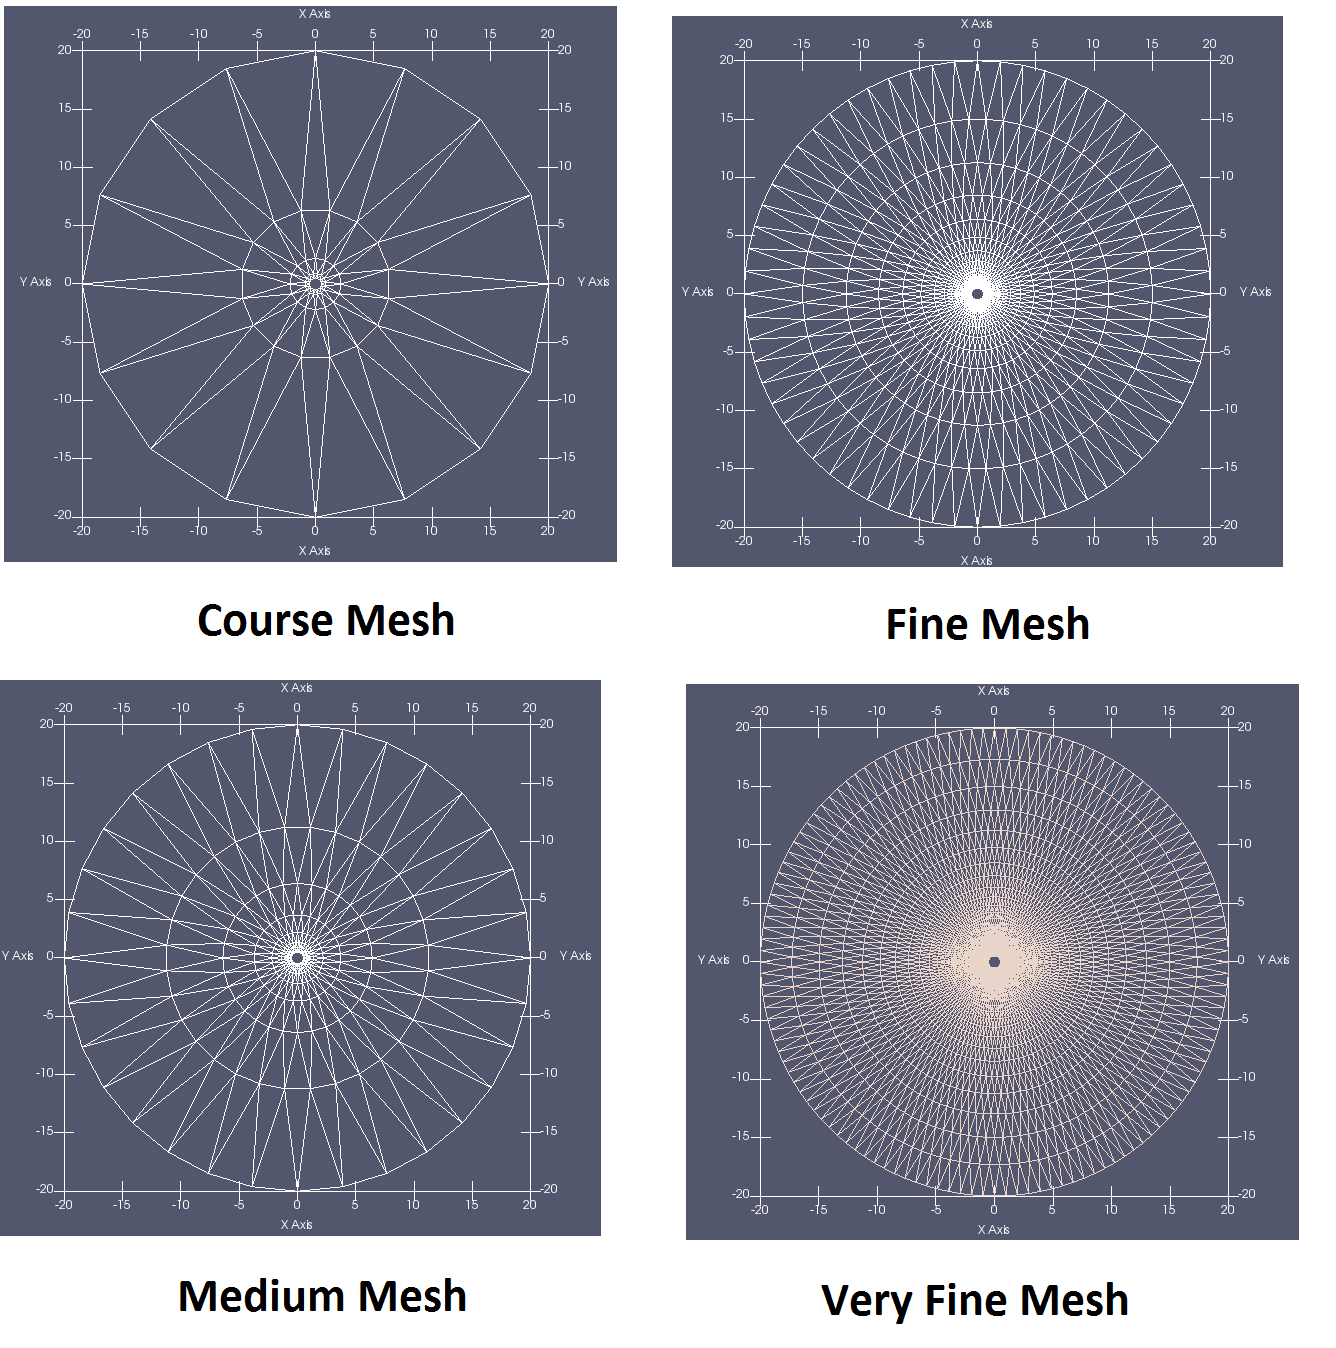
\includegraphics[width=1.0\linewidth]{figure_grid2}}
		%
		\caption{Meshes for determining the order of accuracy}
		\label{cylindergrid}
	\end{figure}
	\clearpage
	Fig. \ref{errorfunction} shows the comparison of error function vs the characteristic grid sizes for different methods. It shows that the entropy production is very high using P0(finite volume) method as there is lot of numerical dissipation and hence the order of accuracy is less than one. Using reconstructed P0P1 method without the limiter, the order of accuracy increases to second order method. It was observed from the simulations that there are lot of oscillations in the solution without the limiter and it induces convergence issues when solving for higher Mach numbers. To avoid it, Van Alberta limiter has been used and it was observed that the order of accuracy has been decreased because of limiting the reconstruction.
	
	\begin{figure}[ht]
		\centering
		\subfigure[Course Mesh]{%
			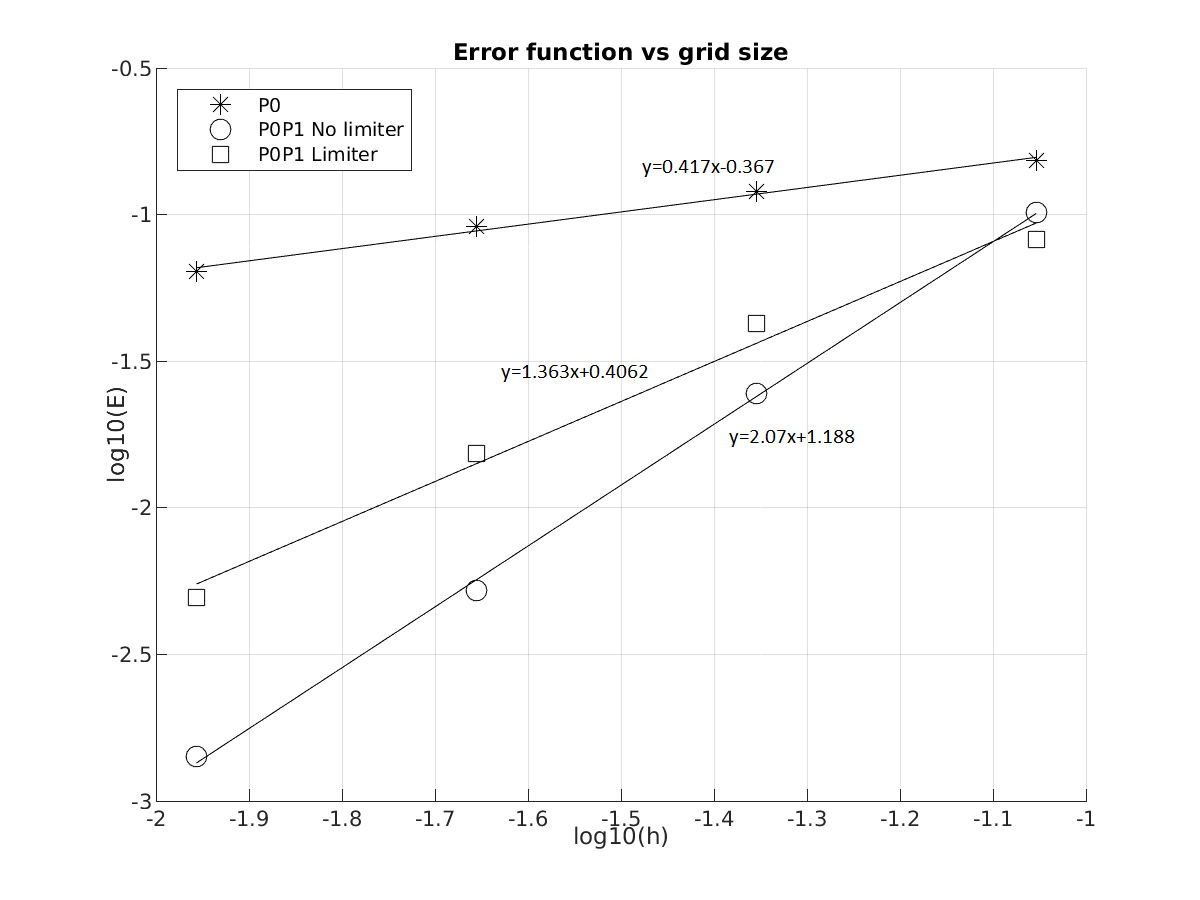
\includegraphics[width=1.0\linewidth]{Errorfunction_2d}}
		%
		\caption{Meshes for determining the order of accuracy}
		\label{errorfunction}
	\end{figure}
	
	To improve the order of accuracy without using limiter, P1 method has been implemented but second order accuracy is not achieved because of bug in the code. However, the required order of accuracy is achieved using reconstruction.
	\clearpage
	
	Fig \ref{figure1}, Fig. \ref{figure2}, Fig. \ref{figure3} shows the comparison of density, pressure and Mach number for four different meshes using P0 method. It can be observed that with mesh refinement, the pressure, density and Mach Number becomes smooth and symmetric about y axis, which is expected for subsonic velocities. However, the solution is not perfectly symmetric even in the fine mesh because the P0 method is dissipative. 
	
	\begin{figure}[ht]
		\centering
		\subfigure[Course Mesh]{%
			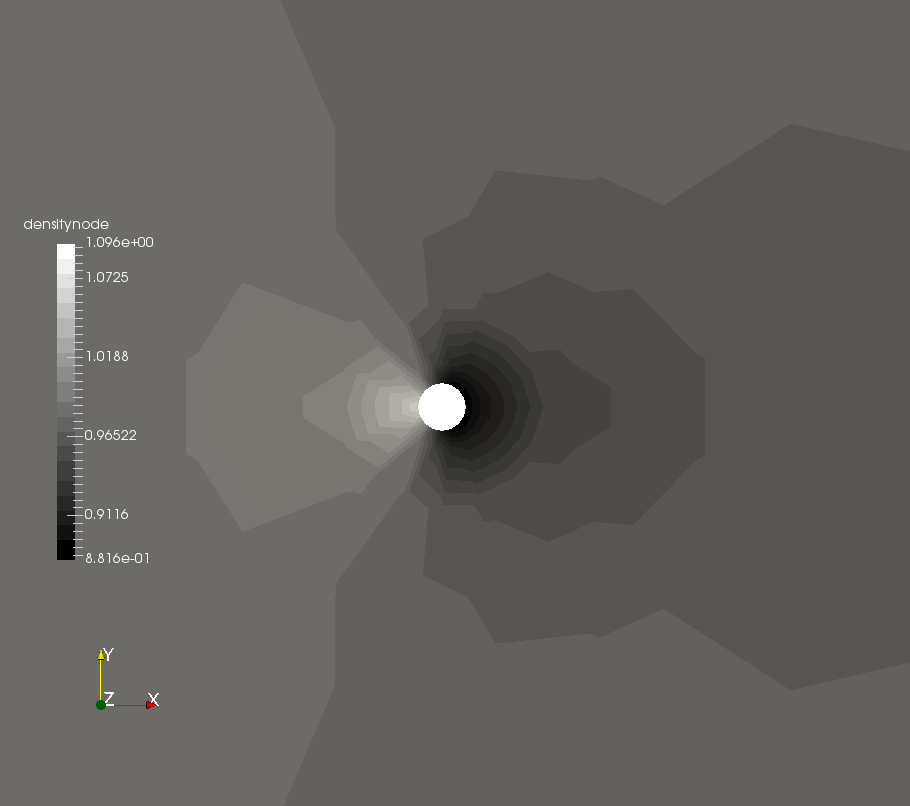
\includegraphics[width=0.45\linewidth]{1density_vcourse_p0}}
		\subfigure[Medium Mesh]{%
			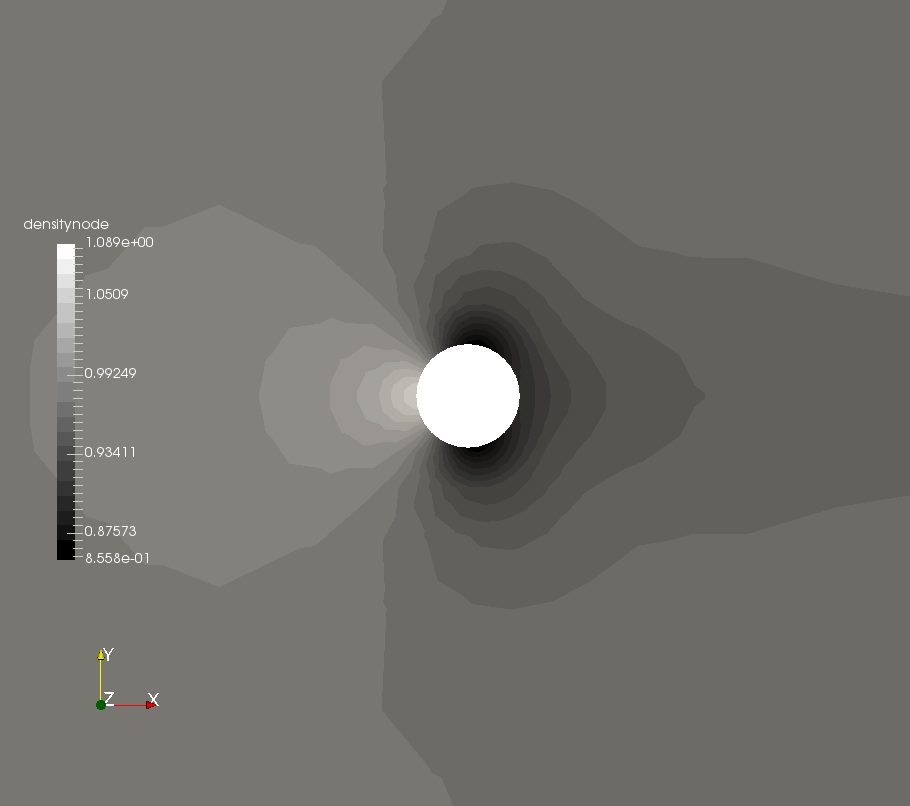
\includegraphics[width=0.45\linewidth]{2density_course_p0}}
		\\
		\subfigure[Fine Mesh]{%
			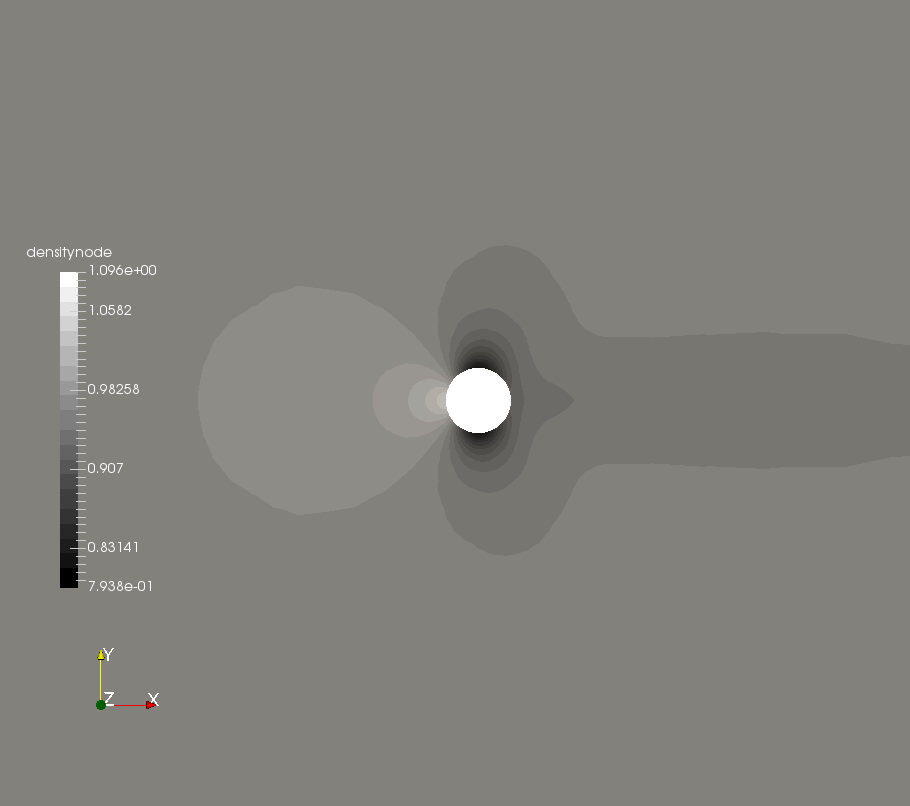
\includegraphics[width=0.45\linewidth]{3density_fine_p0}}
		\subfigure[Very fine Mesh]{%
			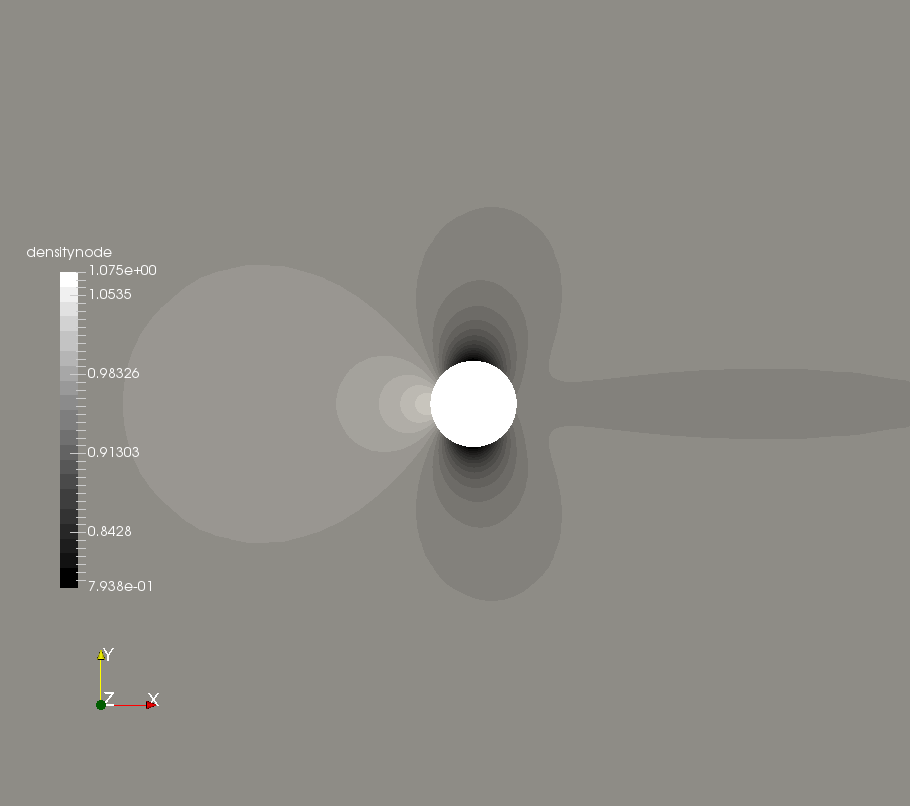
\includegraphics[width=0.45\linewidth]{4density_vfine_p0}}
		%
		\caption{Comparision of density contours for different meshes}
		\label{figure1}
	\end{figure}
	
	
	\begin{figure}[ht]
		\centering
		\subfigure[Course Mesh]{%
			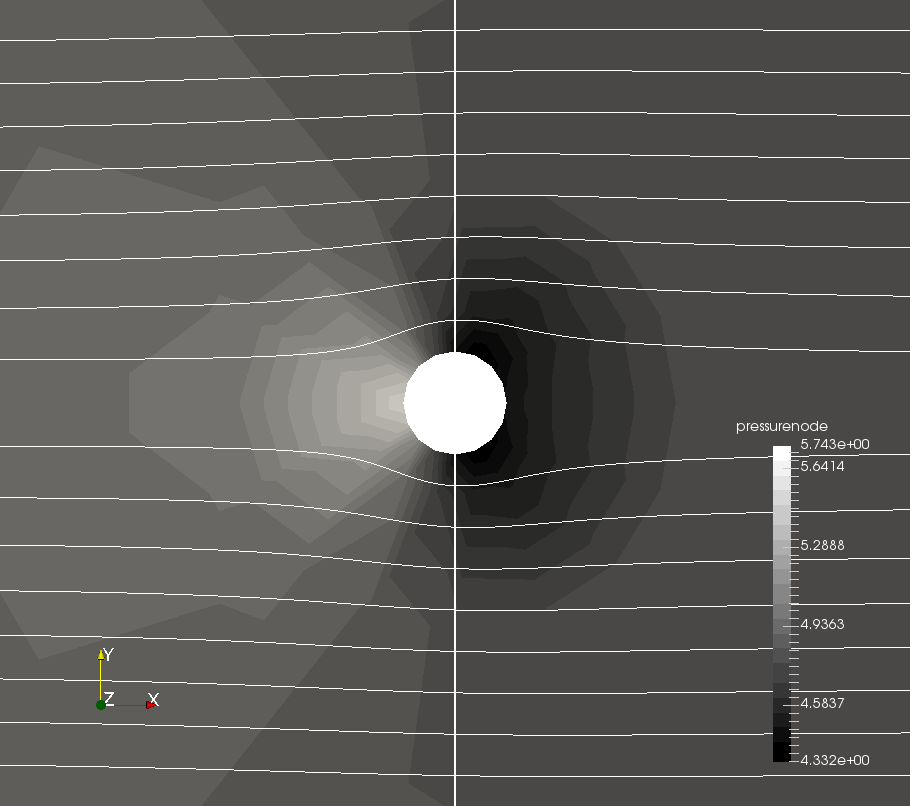
\includegraphics[width=0.45\linewidth]{5pressure_vcourse_p0}}
		\subfigure[Medium Mesh]{%
			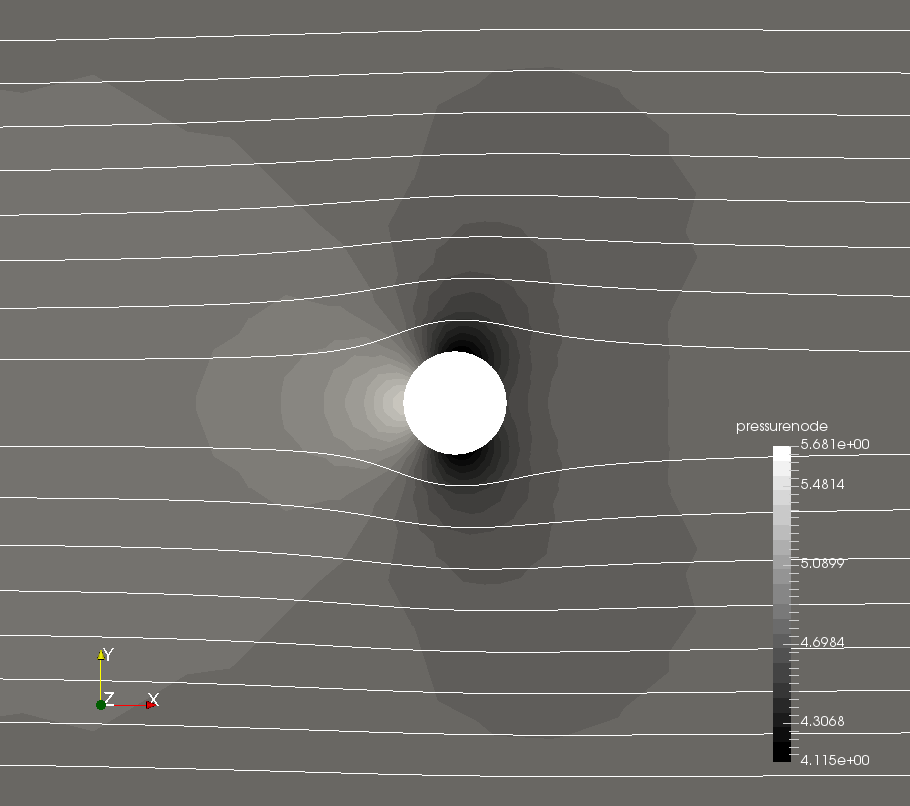
\includegraphics[width=0.45\linewidth]{6pressure_course_p0}}
		\\
		\subfigure[Fine Mesh]{%
			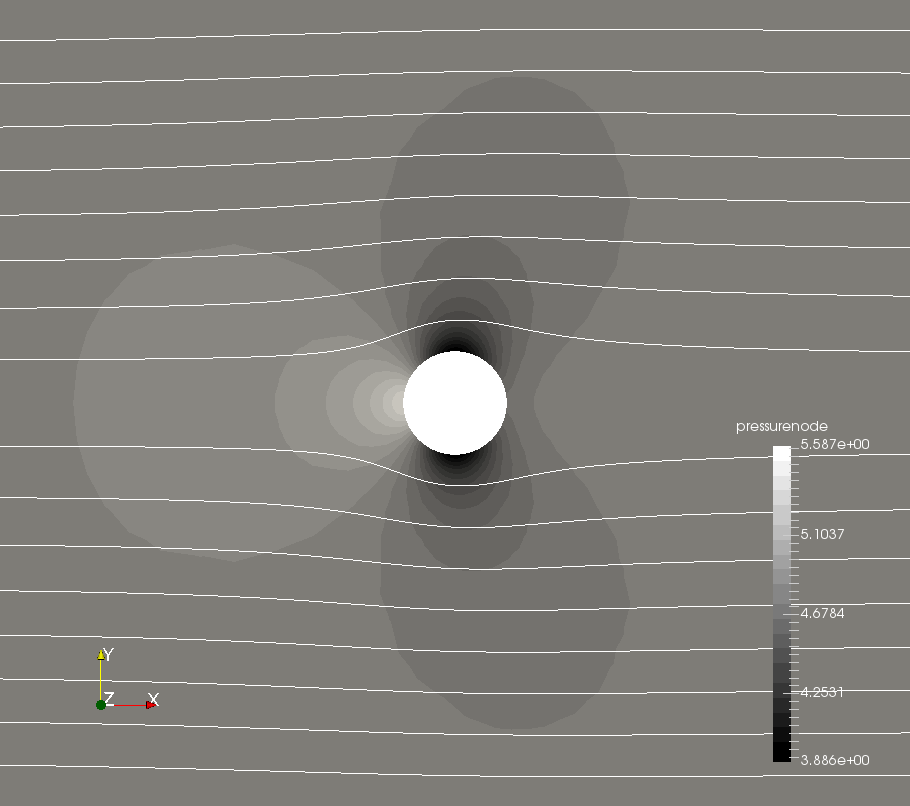
\includegraphics[width=0.45\linewidth]{7pressure_fine_p0}}
		\subfigure[Very fine Mesh]{%
			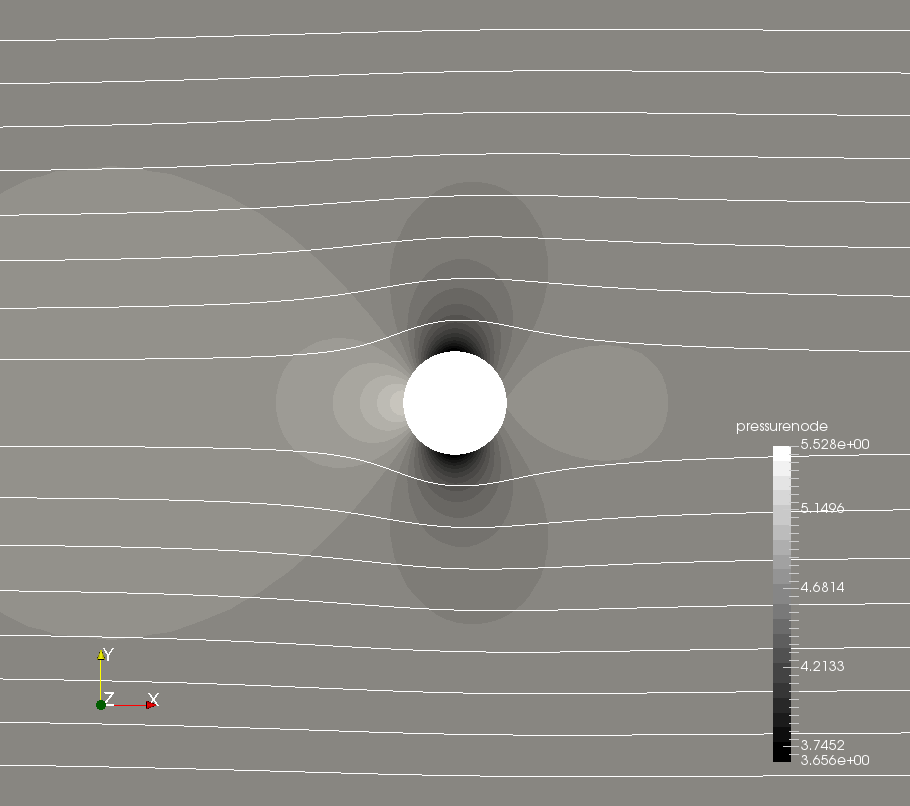
\includegraphics[width=0.45\linewidth]{8pressure_vfine_p0}}
		%
		\caption{Comparision of pressure contours for different meshes}
		\label{figure2}
	\end{figure}
	\clearpage
	The maximum Mach number for flow past a cylinder is 0.7 for fine mesh and it occurs at the top of the cylinder as expected. It can be also observed that the Maximum Mach number increases with mesh refinement. 
	
	\begin{figure}[ht]
		\centering
		\subfigure[Course Mesh]{%
			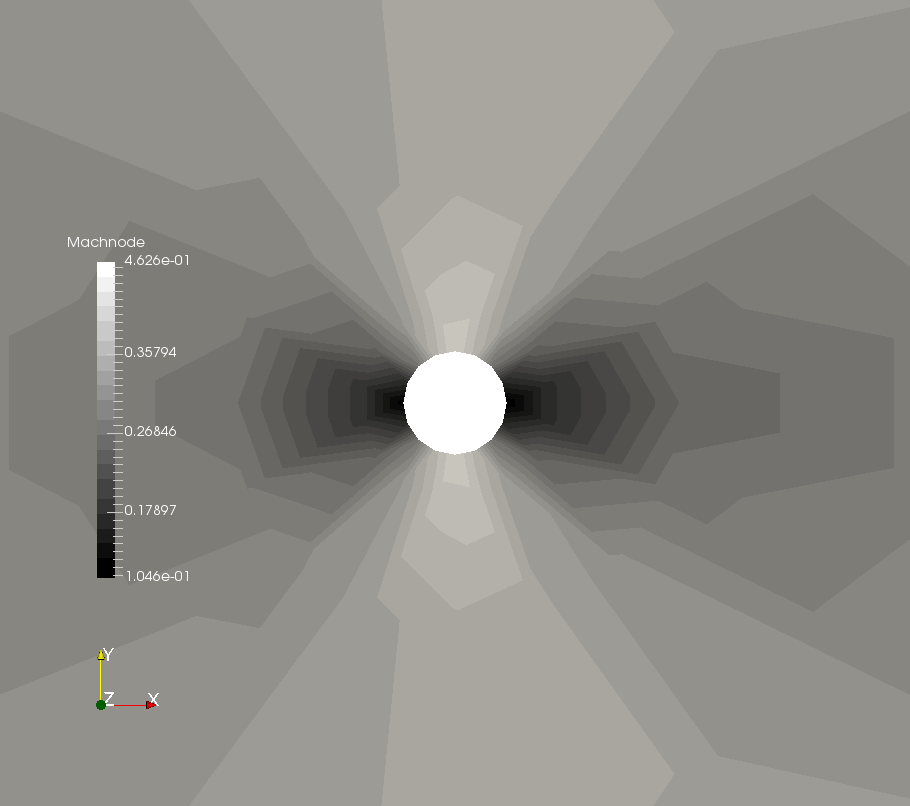
\includegraphics[width=0.45\linewidth]{9Mach_vcourse_p0}}
		\subfigure[Medium Mesh]{%
			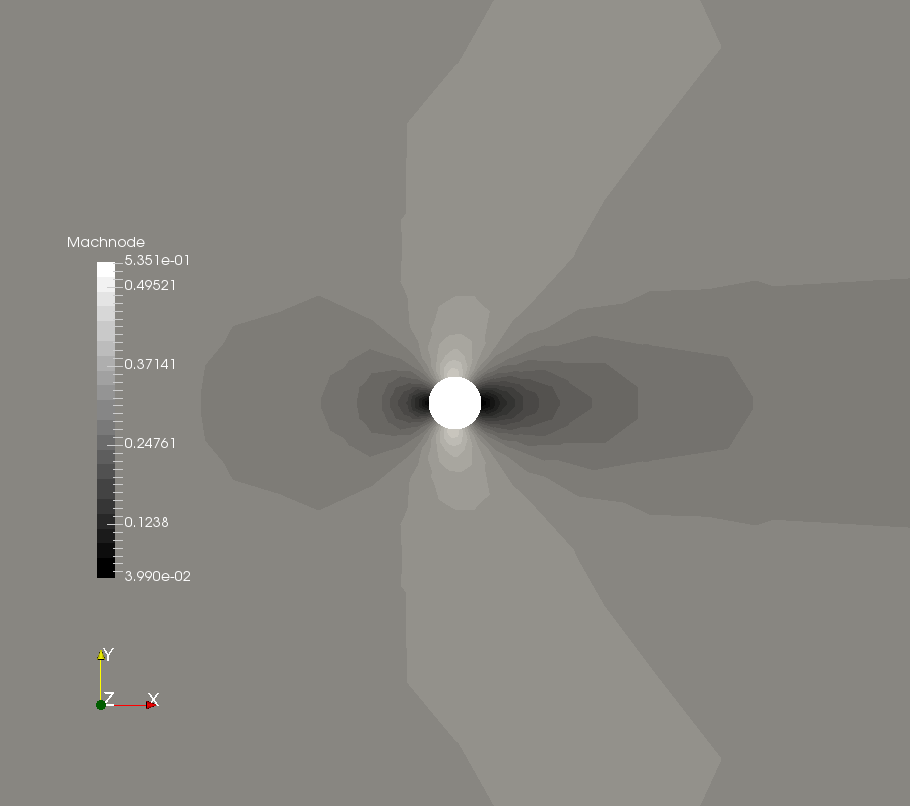
\includegraphics[width=0.45\linewidth]{10Mach_course_p0}}
		\\
		\subfigure[Fine Mesh]{%
			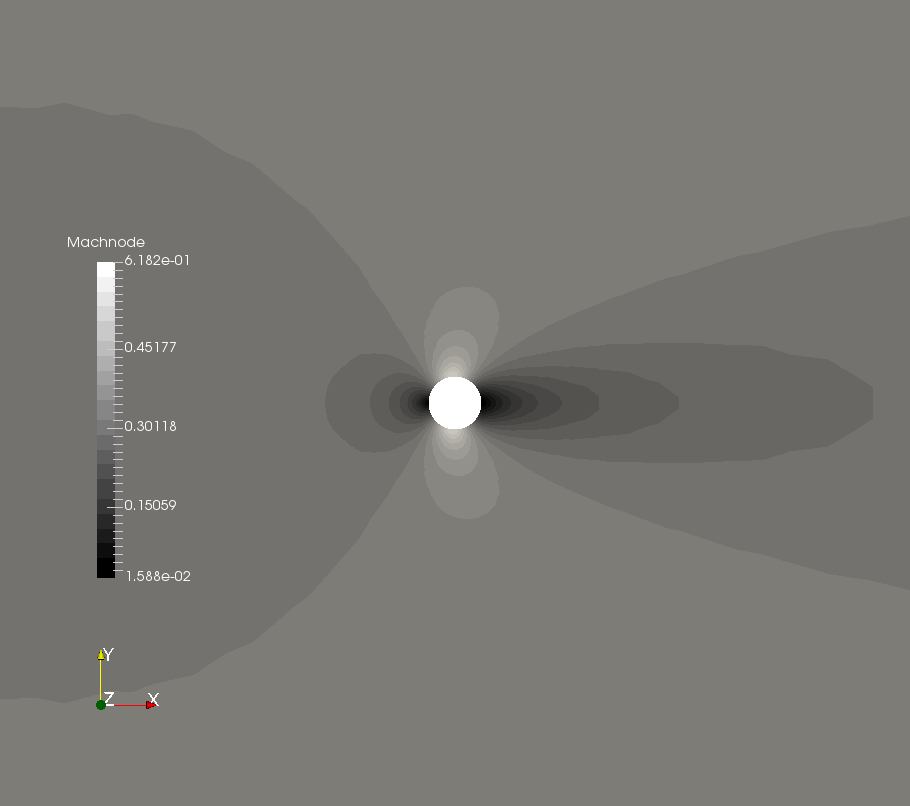
\includegraphics[width=0.45\linewidth]{11Mach_fine_p0}}
		\subfigure[Very fine Mesh]{%
			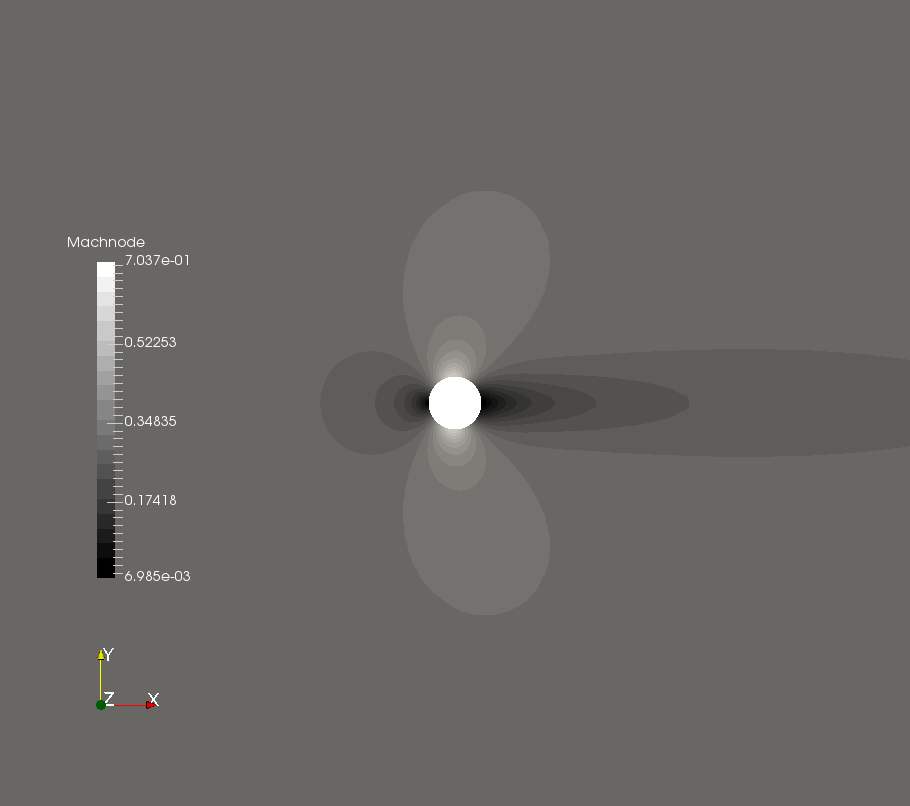
\includegraphics[width=0.45\linewidth]{12Mach_vfine_p0}}
		%
		\caption{Comparision of Mach Number for differen meshes}
		\label{figure3}
	\end{figure}
	\clearpage
	
	Fig. \ref{figure5}, Fig. \ref{figure6} and \ref{figure4} shows the comparison of pressure, Mach number and density on very fine mesh for P0, reconstructed P0P1 without limiter, reconstructed P0P1 with limiter and P1 methods. It can be observed that the solution is almost symmetric about y axis with P0P1 reconstruction without a limiter as the order of accuracy is two and this is expected for a subsonic flow. The P0P1 reconstruction with limiter decreases the accuracy and it is evident from unsymmetrical pressure contours about y axis. 
	\begin{figure}[ht]
		\centering
		\subfigure[P0]{%
			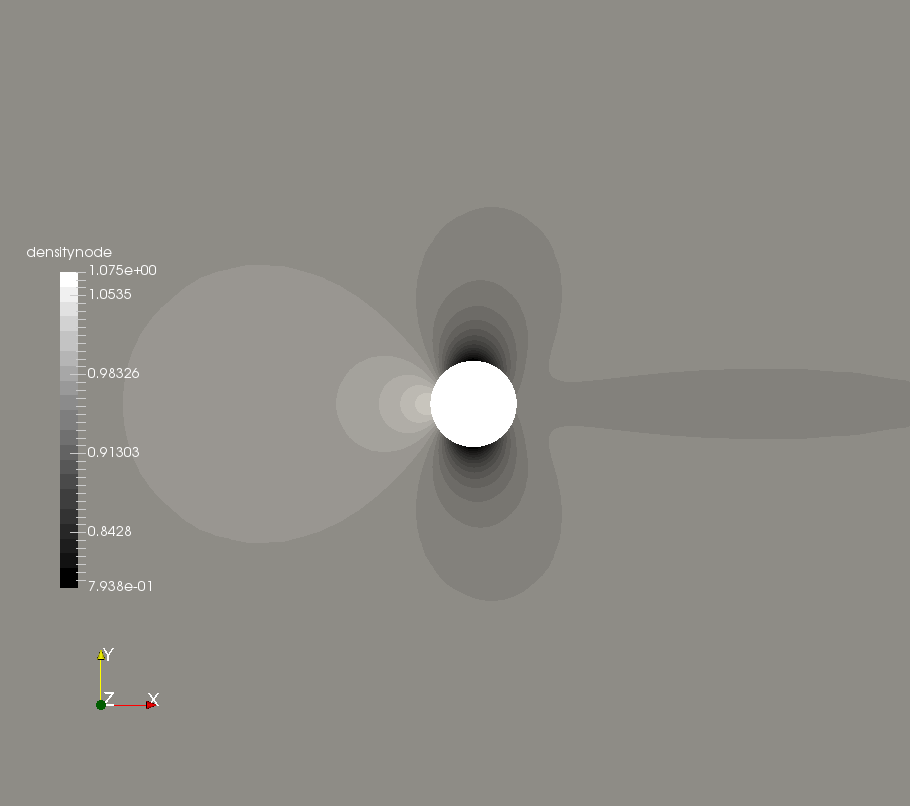
\includegraphics[width=0.45\linewidth]{4density_vfine_p0}}
		\subfigure[P0P1 No Limiter]{%
			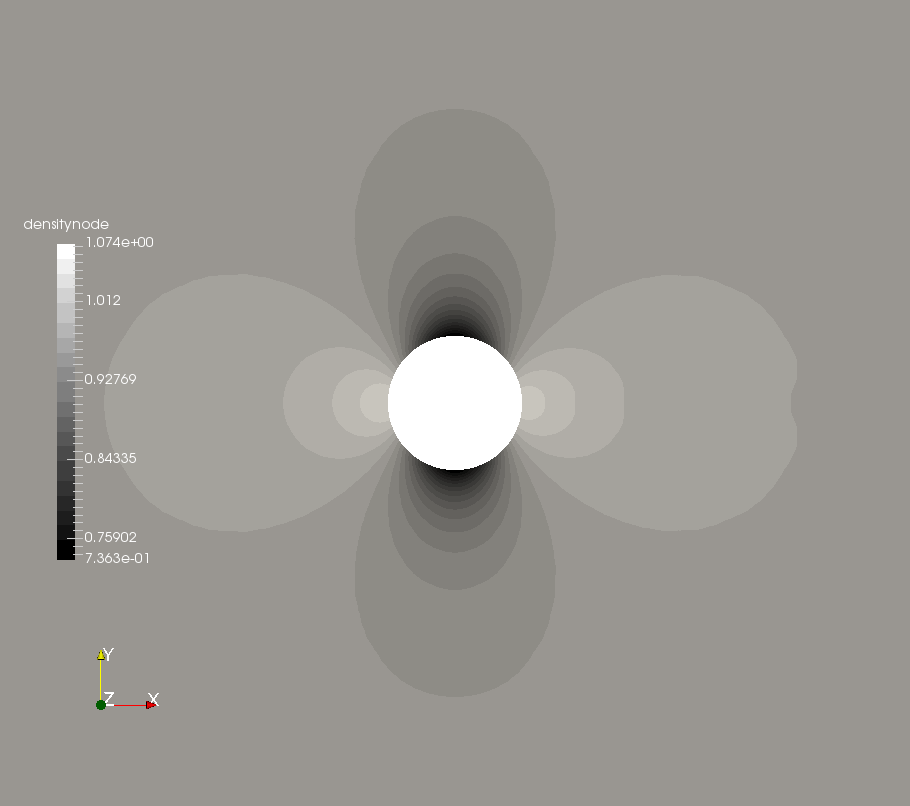
\includegraphics[width=0.45\linewidth]{13density_vfine_p0p1_nolimi}}
		\\
		\subfigure[P0P1 Limiter]{%
			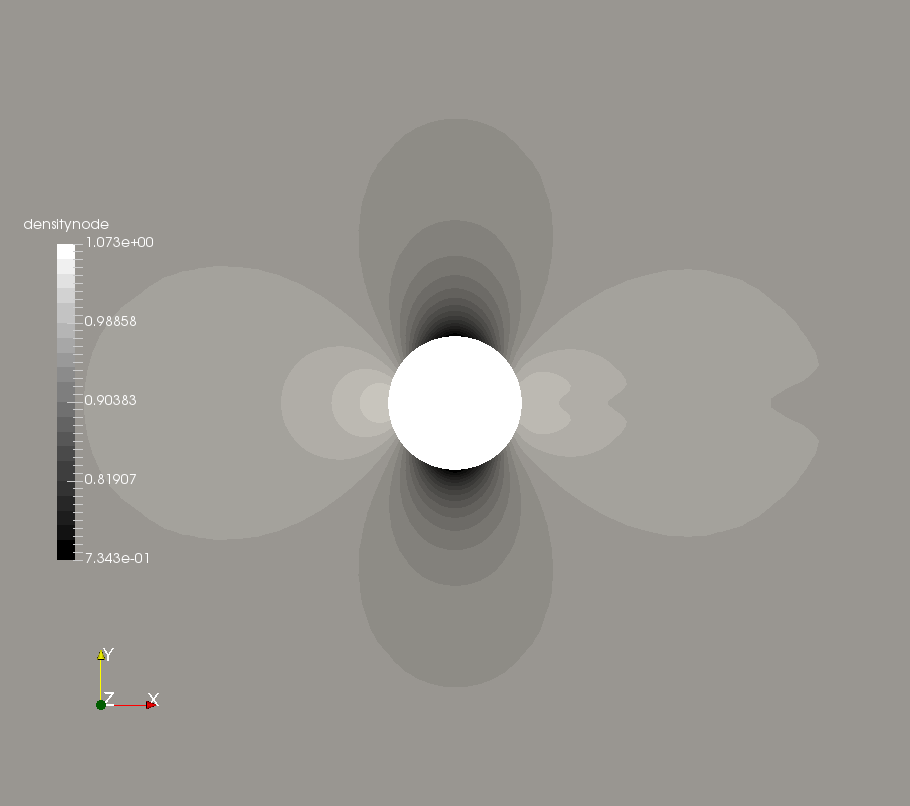
\includegraphics[width=0.45\linewidth]{14density_vfine_p0_limi}}
		\subfigure[P1]{%
			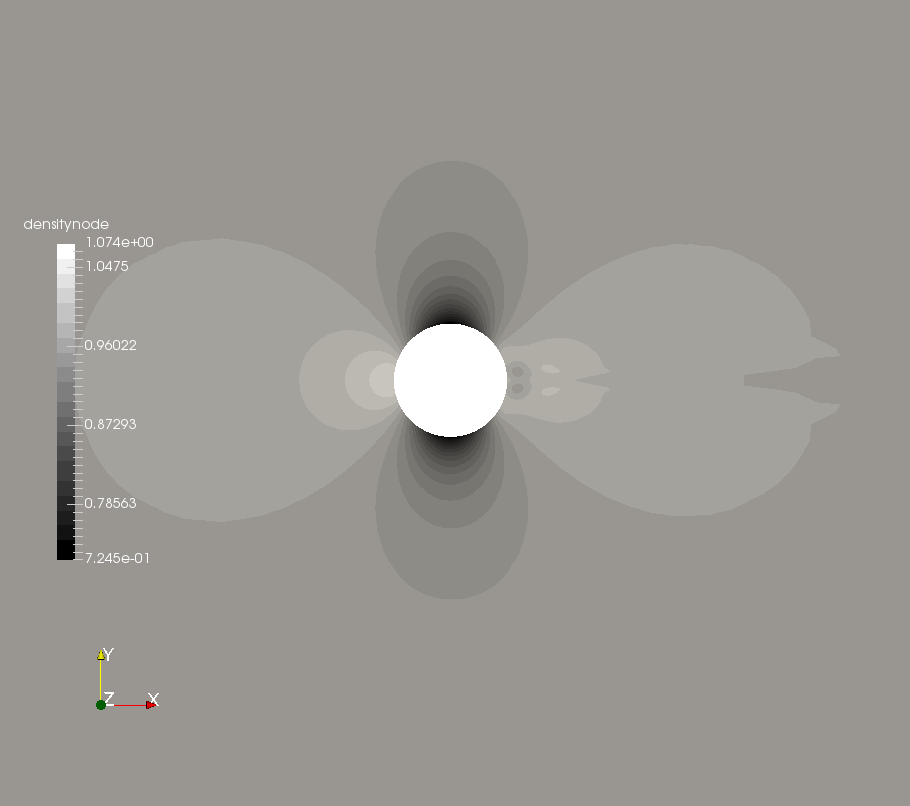
\includegraphics[width=0.45\linewidth]{15density_p1}}
		%
		\caption{Comparision of density contours for different methods}
		\label{figure4}
	\end{figure}
	
	\clearpage
	\subsubsection{Issues with P1 method}
	The order of accuracy for the P1 method is determined to be 1.3  and the reason for this is because of numerical dissipation in the solution caused by bug in the program. This is evident from the circulation behind the cylinder in the streamline plot of P1 solution which generally occurs in case of viscous flows. It was also observed that there is large entropy production near the circulation which is caused by numerical dissipation.  This concludes that the P1 method required to be reviewed to ensure correct results which will improve the order of accuracy. 
	\begin{figure}[ht]
		\centering
		\subfigure[P0]{%
			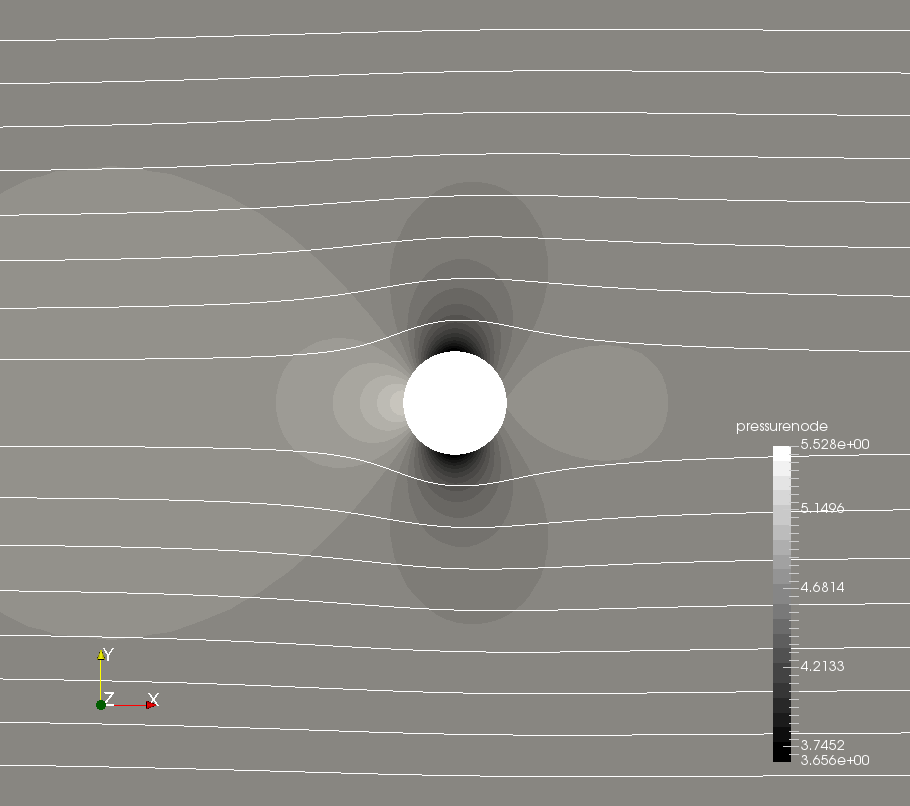
\includegraphics[width=0.45\linewidth]{8pressure_vfine_p0}}
		\subfigure[P0P1 No Limiter]{%
			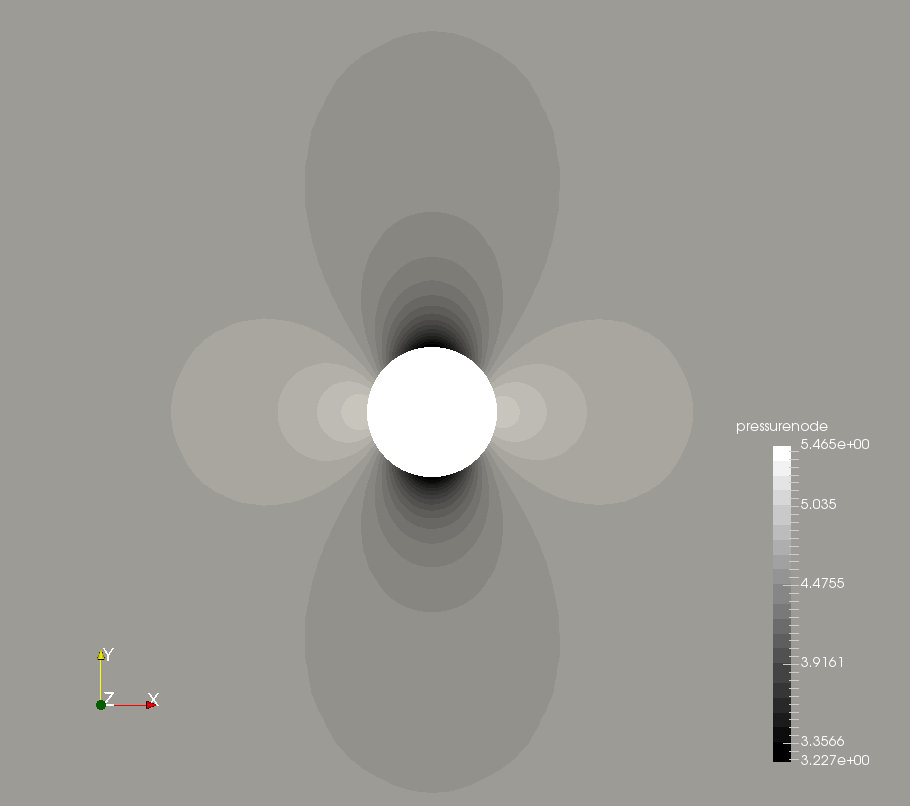
\includegraphics[width=0.45\linewidth]{19pressure_vfine_p0p1_nolimi}}
		\\
		\subfigure[P0P1 Limiter]{%
			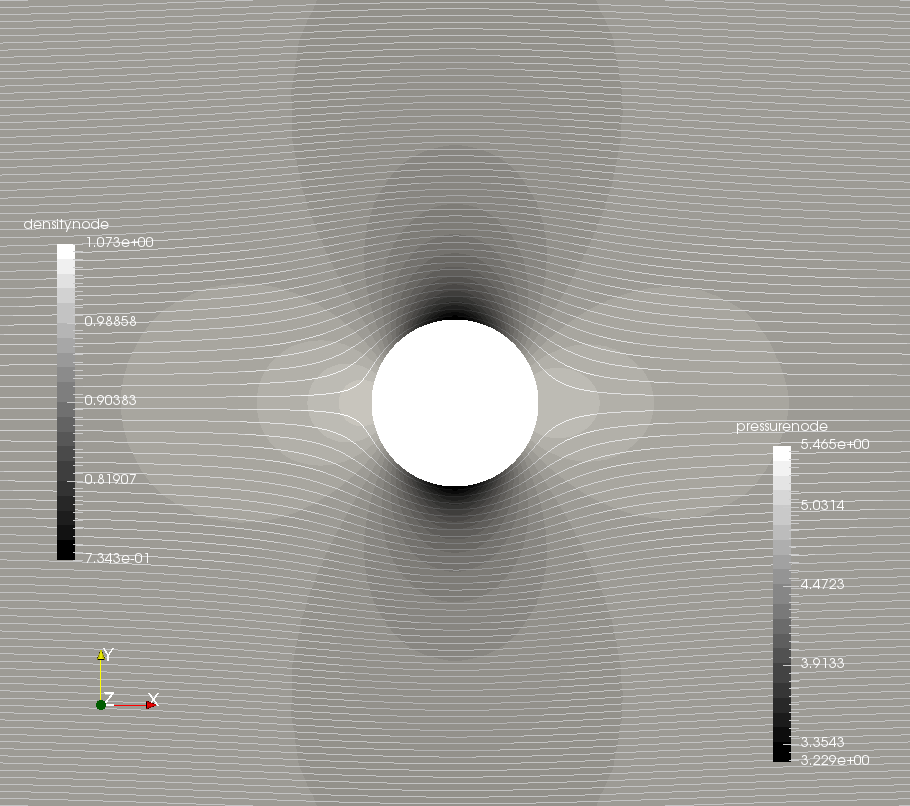
\includegraphics[width=0.45\linewidth]{20pressure_vfine_p0_limi}}
		\subfigure[P1]{%
			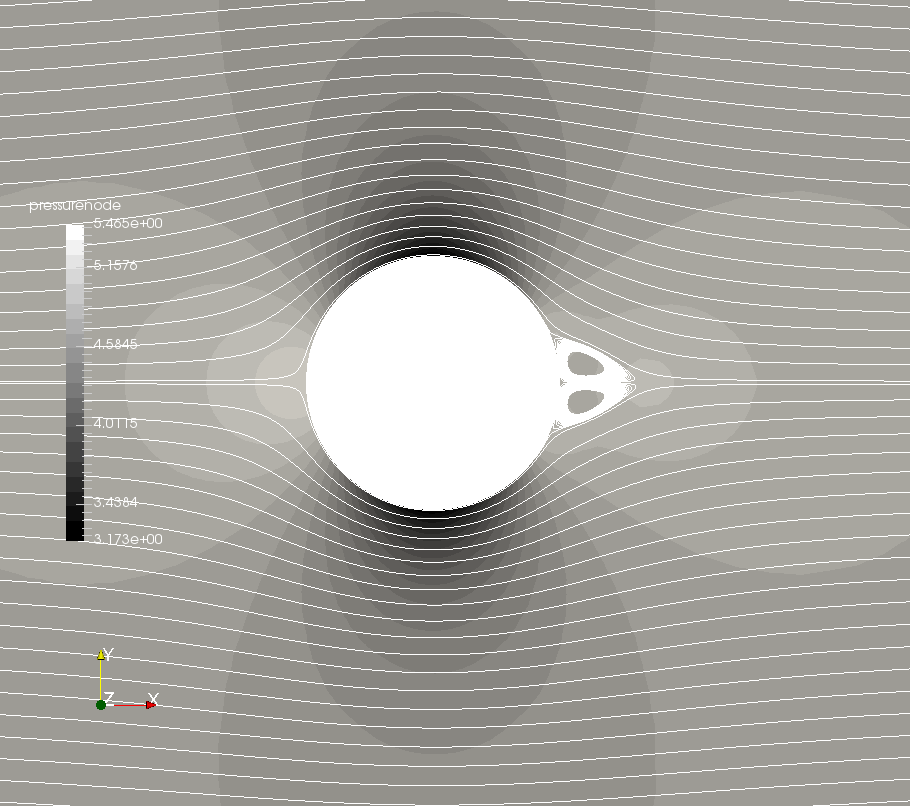
\includegraphics[width=0.45\linewidth]{21pres_p1}}
		%
		\caption{Comparision of pressure contours for different methods}
		\label{figure5}
	\end{figure}
	
	The Mach Number plot shows that the contours are symmetric about y axis without limiter as it is second order accurate and unsymmetrical in all other cases because of numerical dissipation caused by lower order of accuracy.
	
	\begin{figure}[ht]
		\centering
		\subfigure[P0]{%
			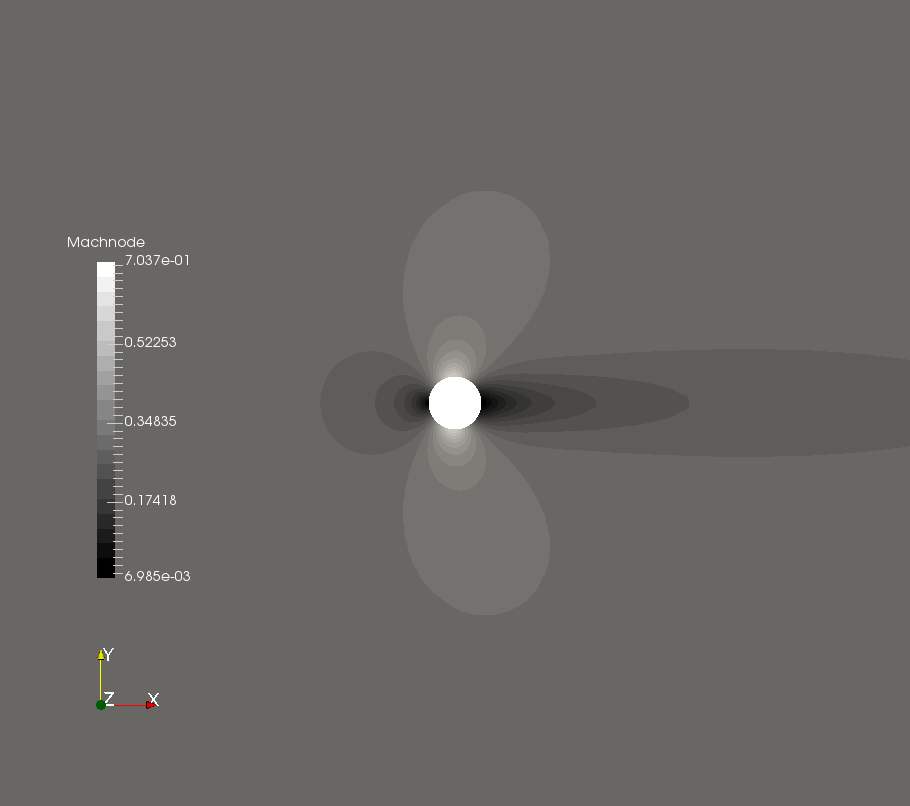
\includegraphics[width=0.45\linewidth]{12Mach_vfine_p0}}
		\subfigure[P0P1 No Limiter]{%
			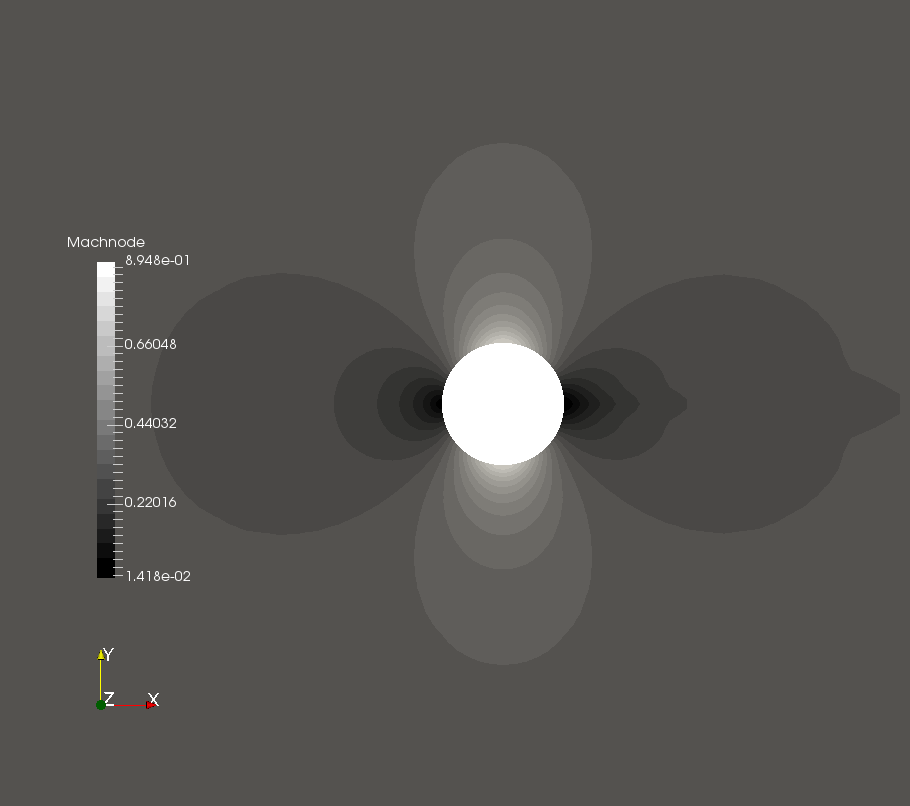
\includegraphics[width=0.45\linewidth]{16Mach_vfine_p0p1_nolimi}}
		\\
		\subfigure[P0P1 Limiter]{%
			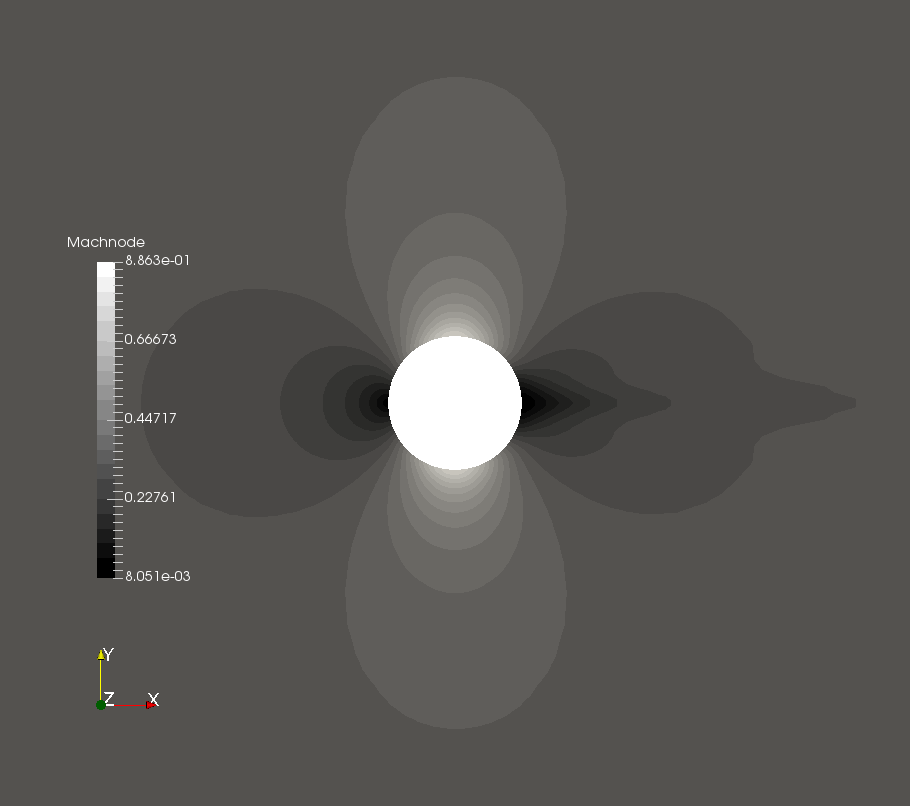
\includegraphics[width=0.45\linewidth]{17Mach_vfine_p0_limi}}
		\subfigure[P1]{%
			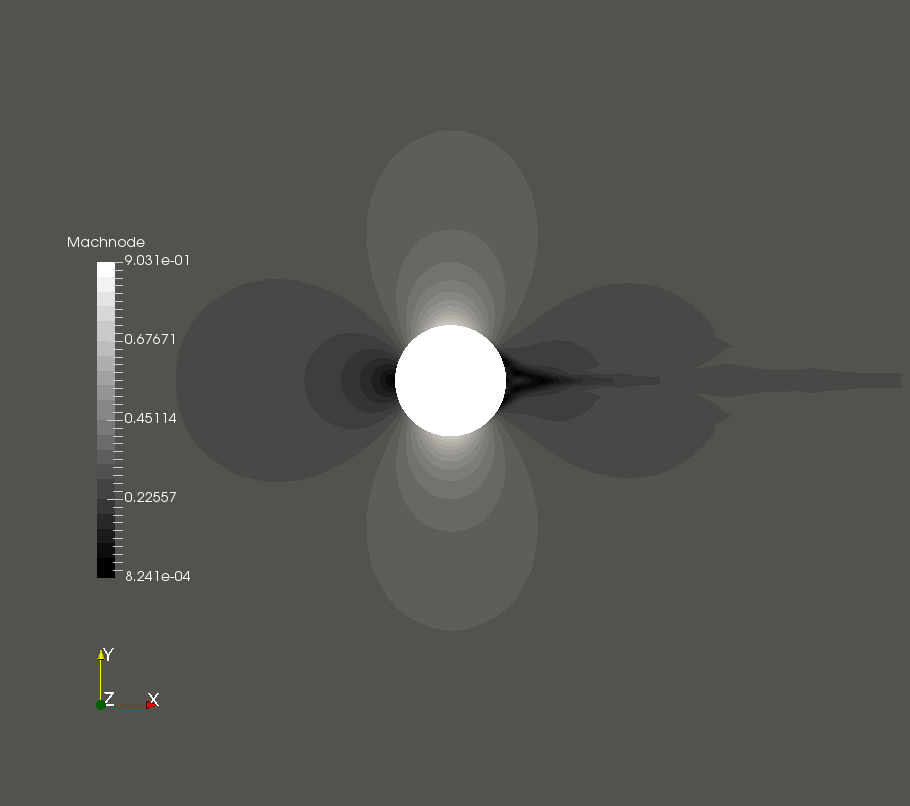
\includegraphics[width=0.45\linewidth]{18Mach_p1}}
		%
		\caption{Comparision of Mach number for different methods}
		\label{figure6}
	\end{figure}
	
	\subsubsection{Convergence plot}
	Fig. \ref{figure7} shows the plot of Residues vs the iteration number. The relative residue is the ratio of absolute residue at current iteration and absolute residue after first iteration. The solution is considered to be converged when the relative residue is 1e-6. It can be observed from the plot that relative residue of continuity, momentum, energy follows almost similar trend with slightly more number of iteration for relative residue of mass to reach the tolerance (1e-6) and hence mass residue plots are compared for subsequent cases. Fig. \ref{figure7}.c  and d shows the comparison of convergence plots for different meshes. It can be observed from the plot that the very fine mesh take more number of iterations to converge and absolute residue for all the meshes is around 1e-10. Fig \ref{figure7}.e and \ref{figure7}, shows the comparison of convergence plots for different methods on very fine mesh. It is observed that all the cases take similar number of iterations to converge.
	
	\begin{figure}[ht]
		\centering
		\subfigure[Absolute Residue]{%
			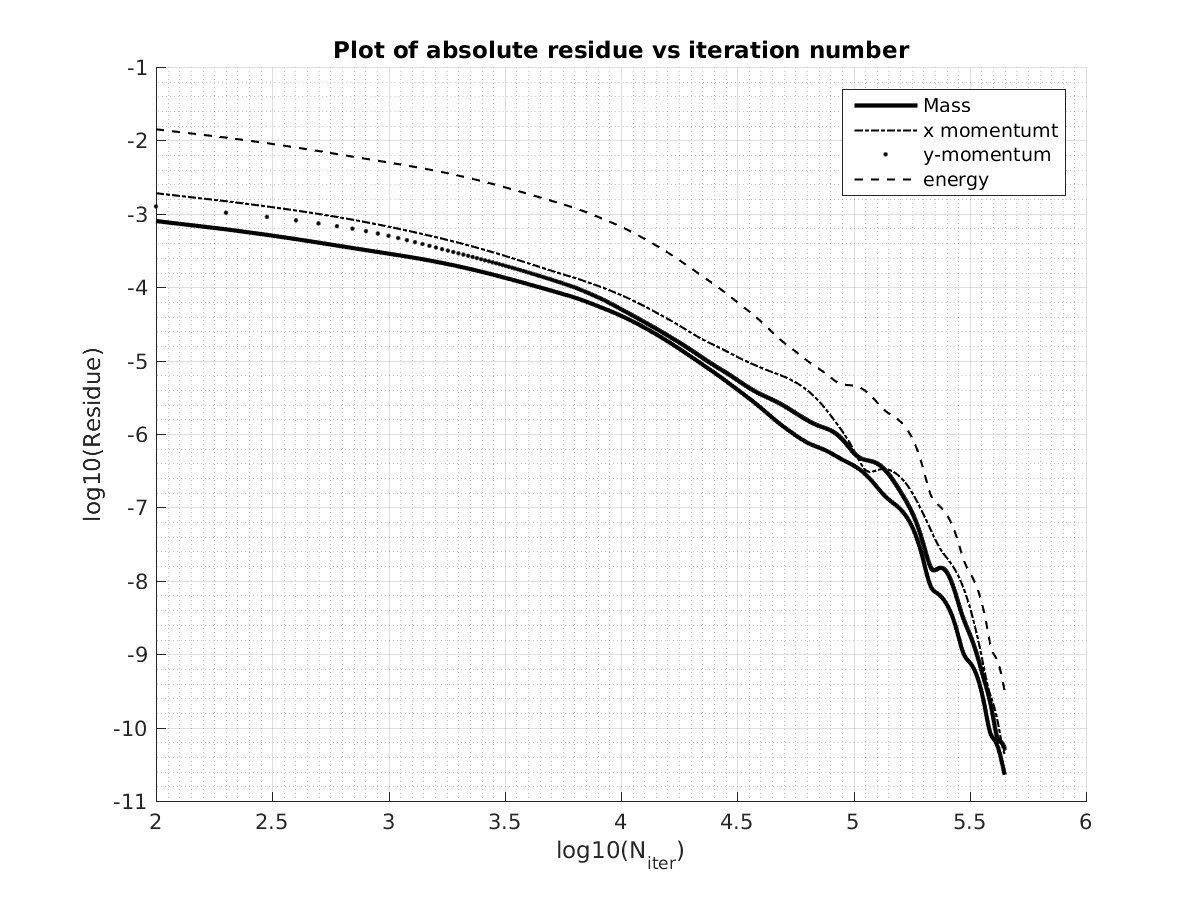
\includegraphics[width=0.45\linewidth]{22absresid_vfine}}
		\subfigure[Relative Residue]{%
			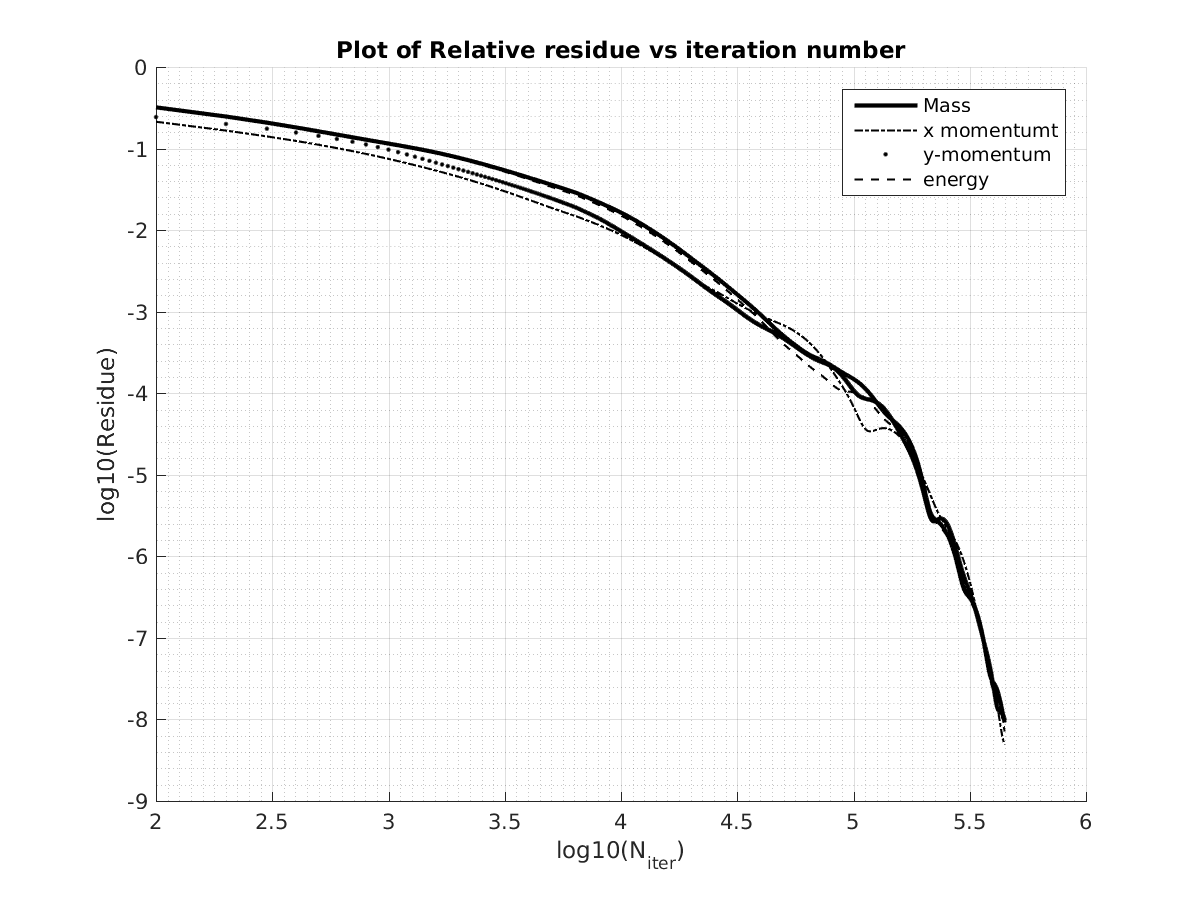
\includegraphics[width=0.45\linewidth]{23relresid_vfine}}
		\\
		\subfigure[Absolute Residue]{%
			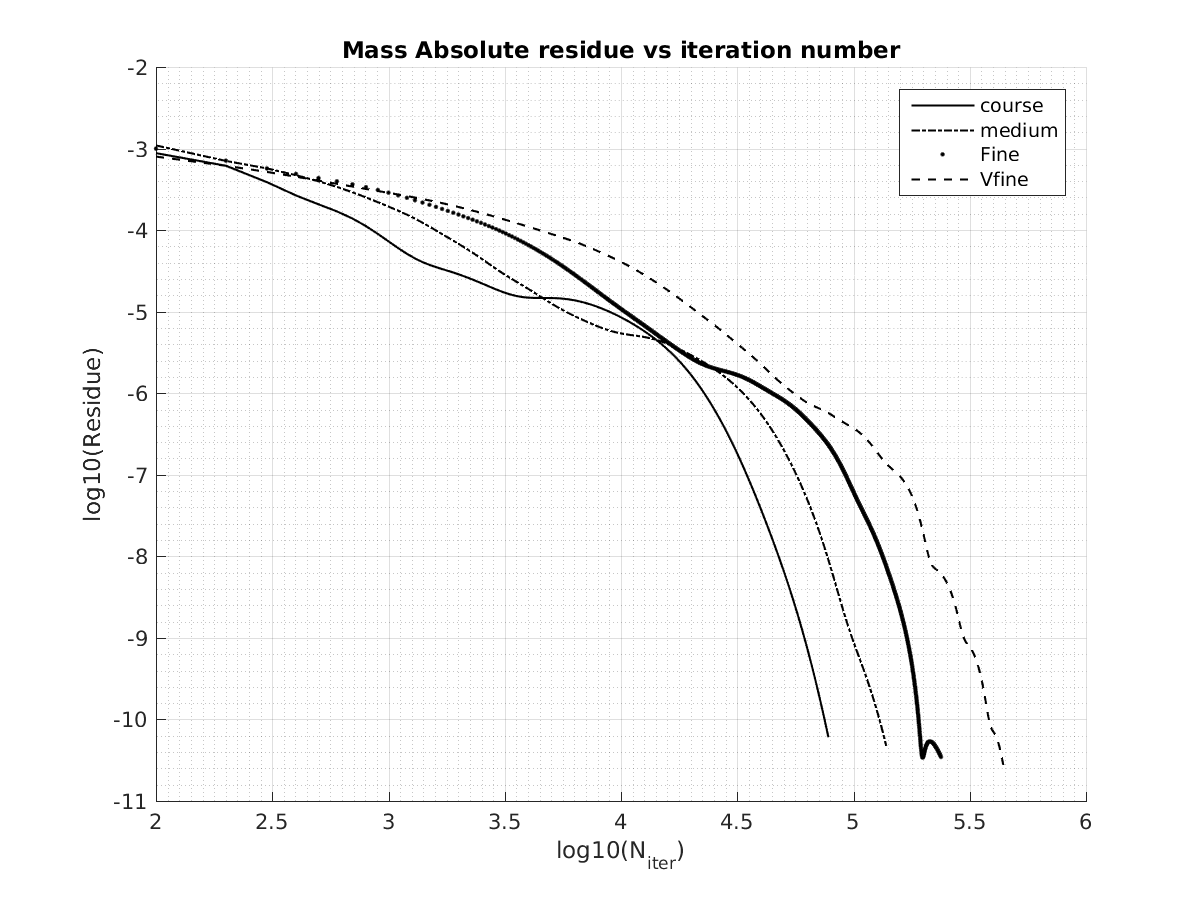
\includegraphics[width=0.45\linewidth]{24absresid_allmesh}}
		\subfigure[Relative Residue]{%
			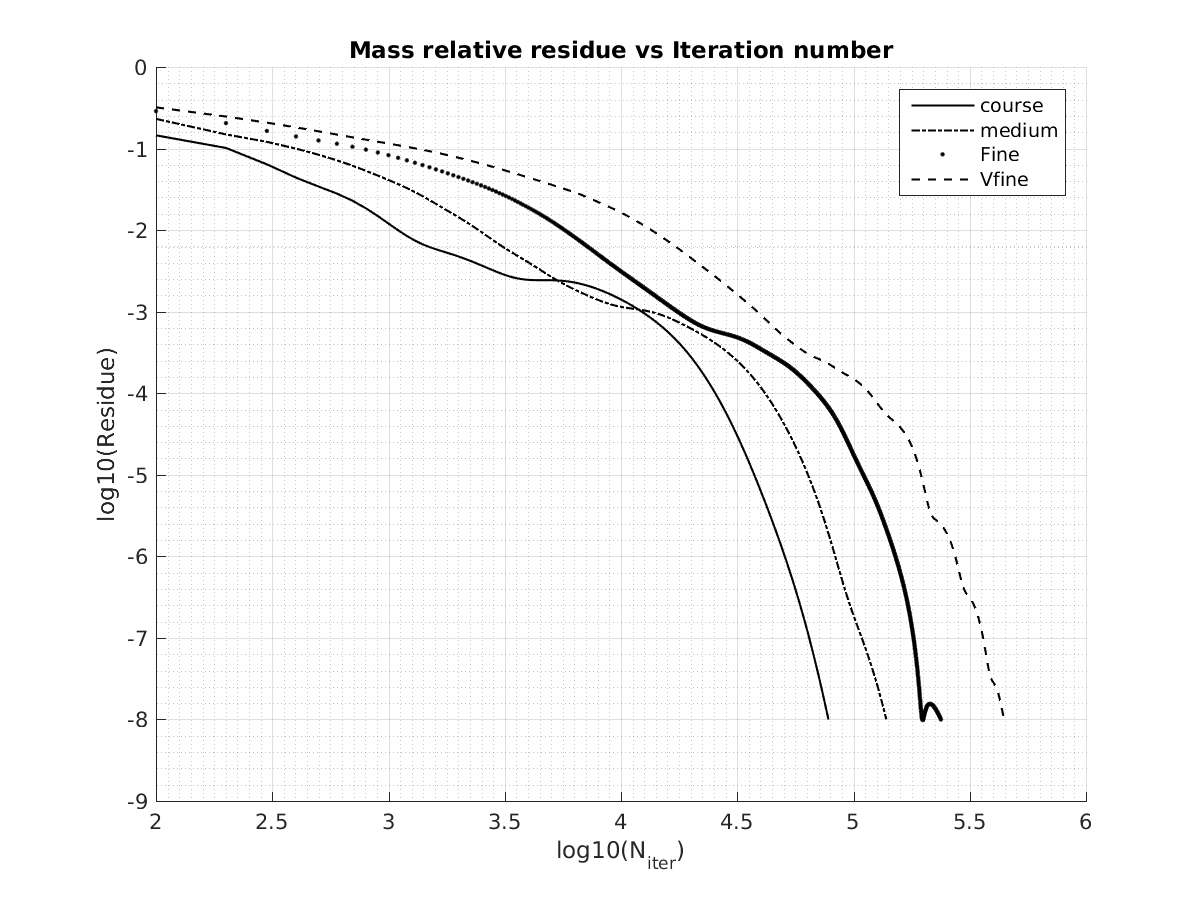
\includegraphics[width=0.45\linewidth]{25relresid_allmesh}}
		\\
		\subfigure[Absolute Residue]{%
			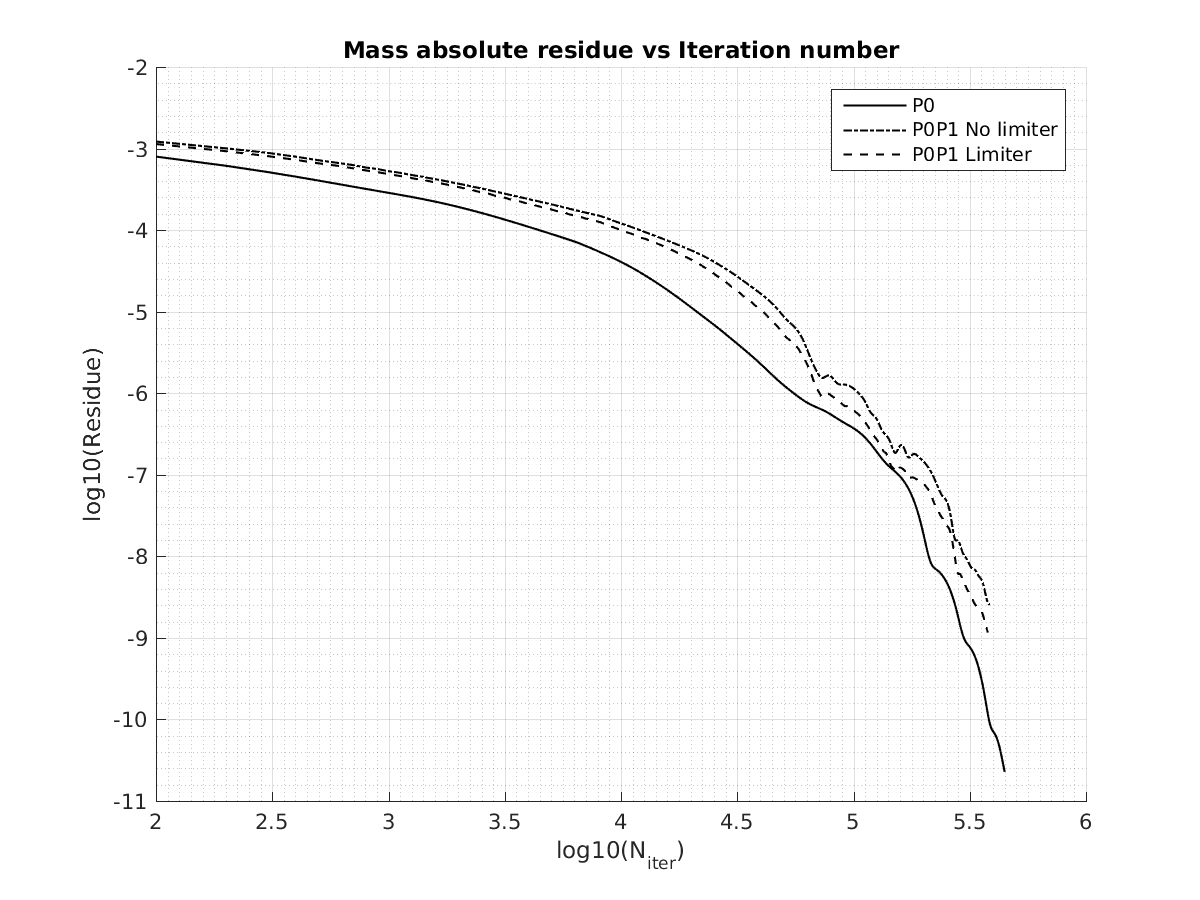
\includegraphics[width=0.45\linewidth]{26cyl_abs_res_comp}}
		\subfigure[Relative Residue]{%
			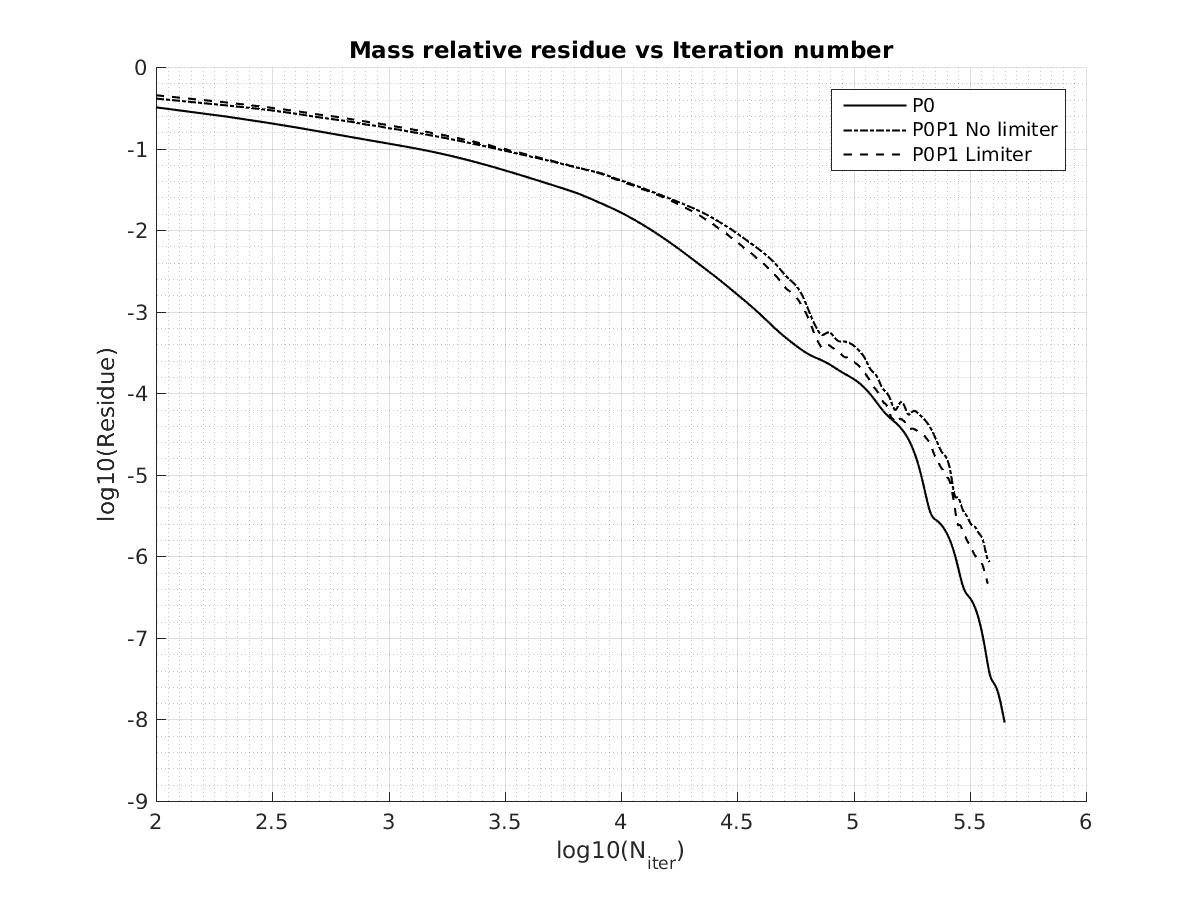
\includegraphics[width=0.45\linewidth]{27cyl_rel_res_comp}}
		%
		\caption{Comparision of Residues for flow past a cylinder}
		\label{figure7}
	\end{figure}
	
	\clearpage
	\subsection{Transonic flow past NACA airfoil (M=0.85)}
	The second case is flow past an airfoil with free stream Mach number of 0.85 at 1 degree angle of attack. Fig. \ref{airfoil} shows the grid near the airfoil.
	
	\begin{figure}[ht]
		\centering
		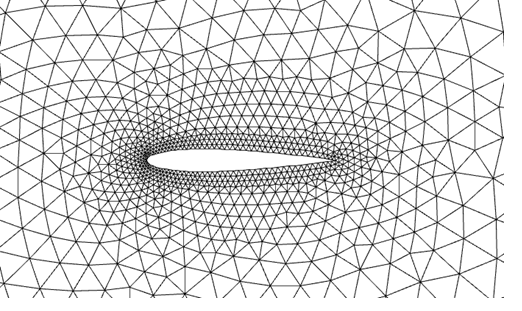
\includegraphics[width=0.45\linewidth]{airfoil}
		\caption{Comparision of flow inside internal flow}
		\label{airfoil}
	\end{figure}
	
	The simulation is conducted using P0, reconstructed P0P1 without limiter and with limiter. Fig. \ref{densitynaca} and \ref{figure9} shows the comparison of density, pressure and Mach number for all the three cases. It can be observed that the solution is not symmetric about the x axis because of finite angle of attack.\newline
	\newline
	The contour plots shows that the density, pressure is maximum and Mach number is minimum at the nose of the airfoil. Pressure and density decreases over the airfoil whereas the Mach number increase due to decrease in cross-section. Finally there is a shock near the trailing edge of the airfoil where density,  pressure increases and Mach number decreases. Comparing the solutions of all the methods it can be observed that shock is sharp in case of reconstruction compared to P0 Case. However, there are oscillation without the limiter and oscillations are reduced with the limiter. This is evident from the fig \ref{figure9}.g and \ref{figure9}.h.
	
	\begin{figure}[ht]
		\centering
		\subfigure[Density P0]{%
			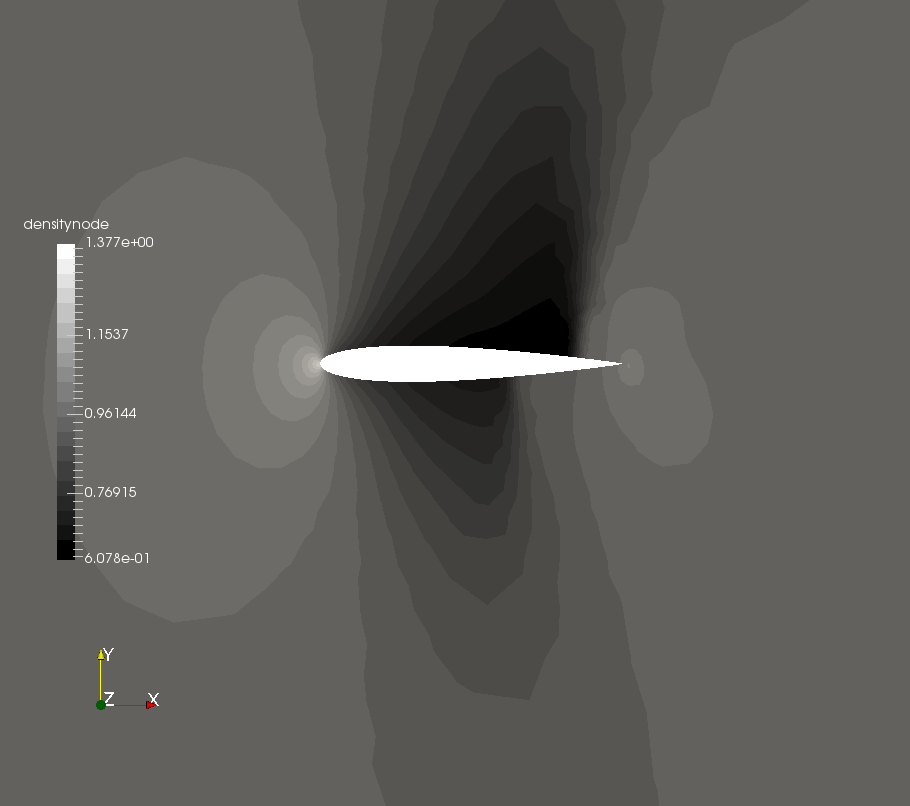
\includegraphics[width=0.4\linewidth]{34density_p0_naca}}
		\subfigure[Density P0P1 with Limiter]{%
			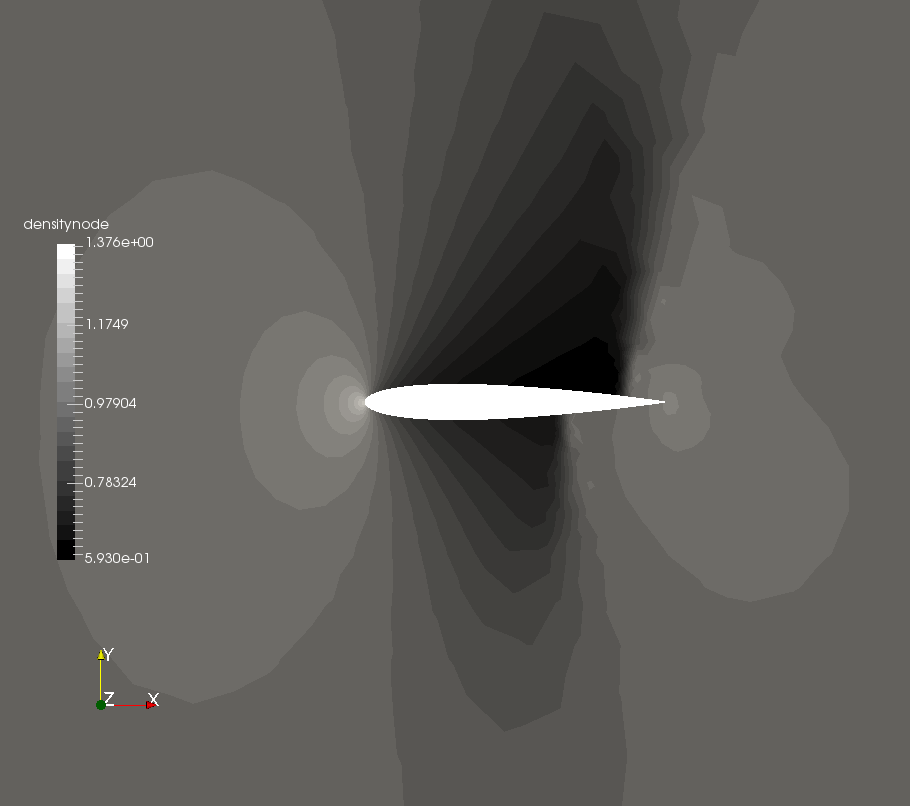
\includegraphics[width=0.4\linewidth]{35density_p0p1_naca}}
		%
		\caption{Solution of NACA airfoil}
		\label{densitynaca}
	\end{figure}
	
	\begin{figure}[ht]
		\centering
		\subfigure[Pressure P0]{%
			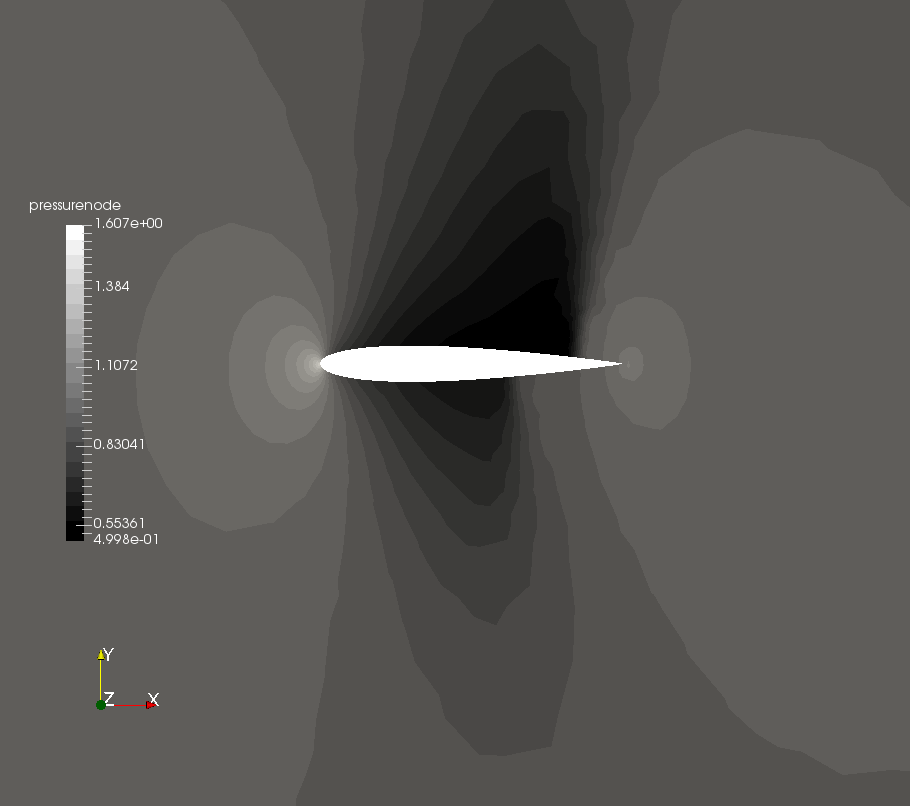
\includegraphics[width=0.4\linewidth]{37pres_p0_naca}}
		\subfigure[Pressure P0P1]{%
			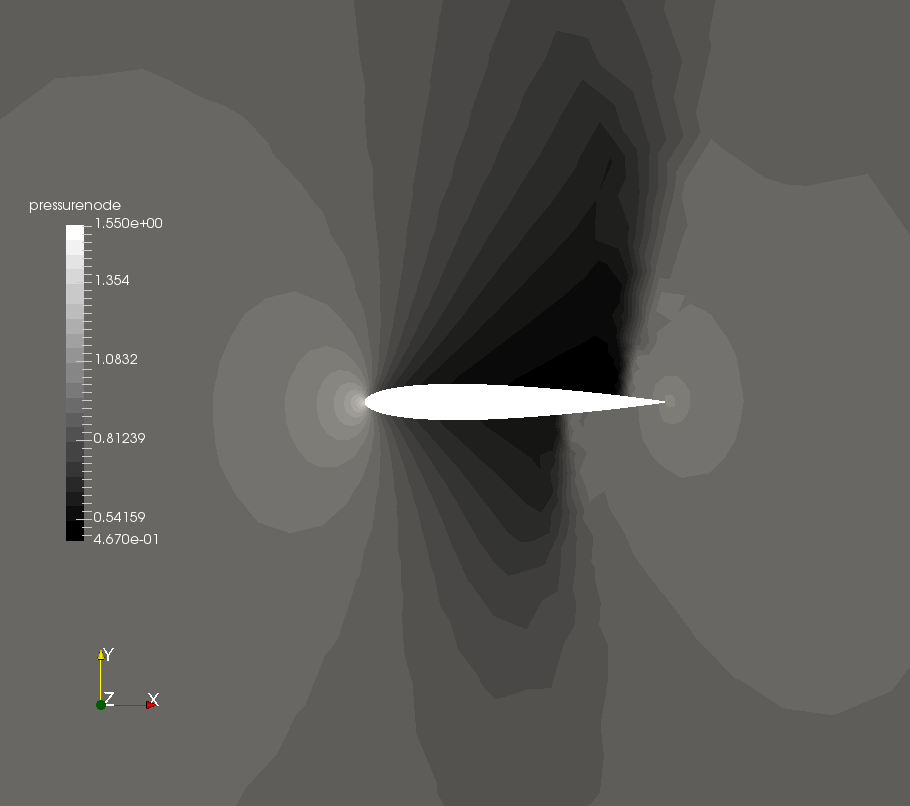
\includegraphics[width=0.4\linewidth]{38pres_p0p1_naca}}
		\subfigure[Pressure P0P1 with Limiter]{%
			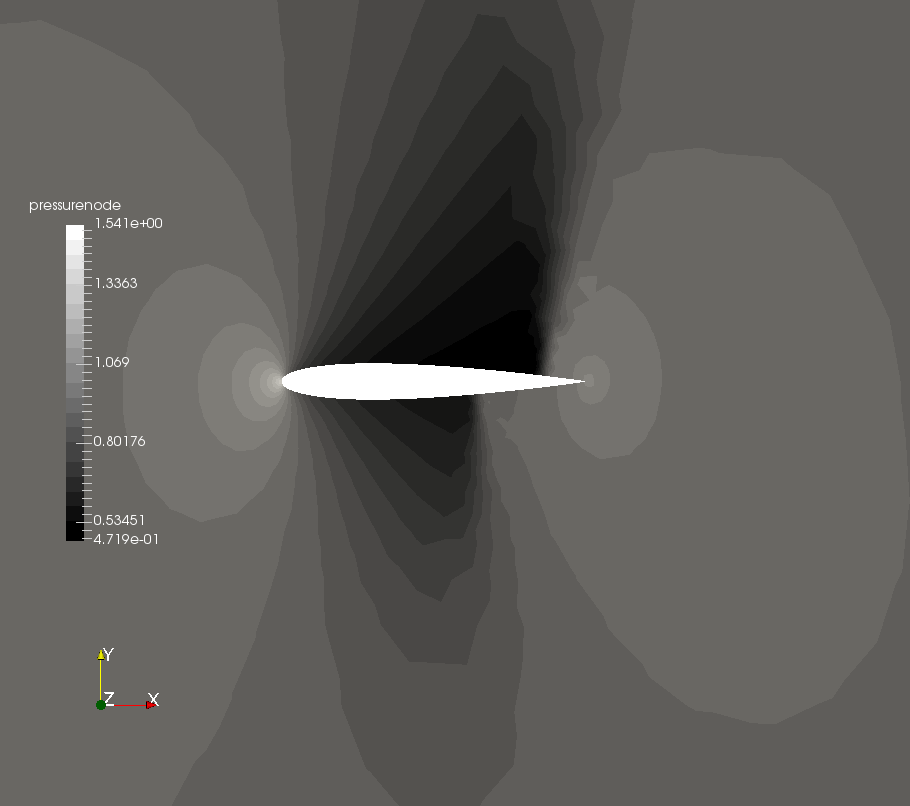
\includegraphics[width=0.4\linewidth]{39pres_p0p1_limi_naca}}
		\subfigure[Mach P0]{%
			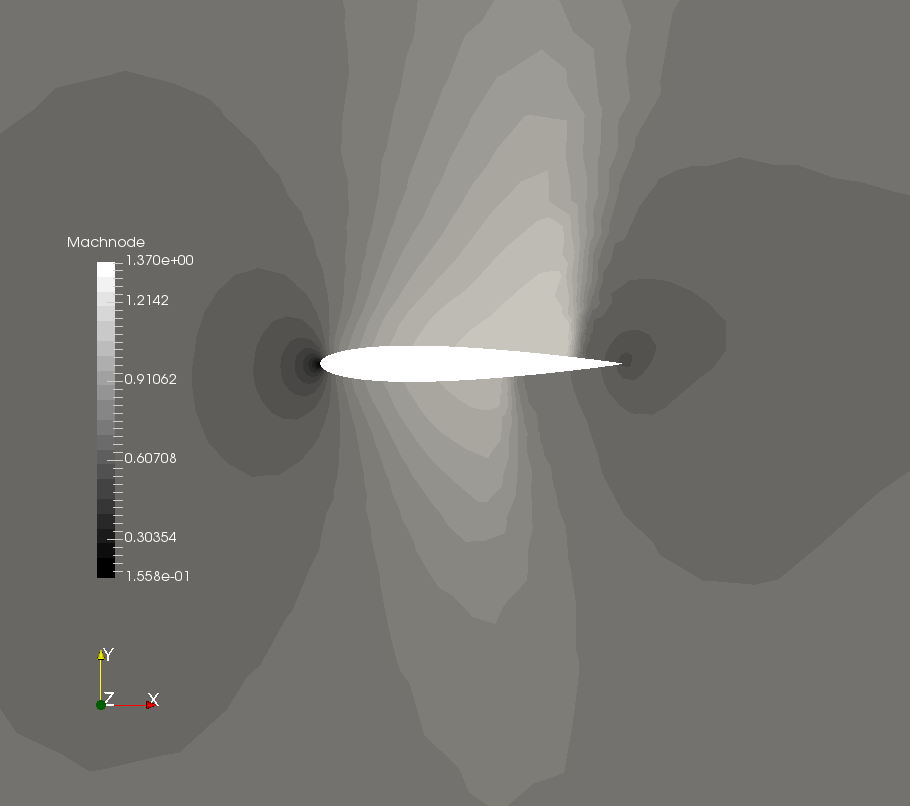
\includegraphics[width=0.4\linewidth]{40Mach_p0_naca}}
		\subfigure[Mach P0P1]{%
			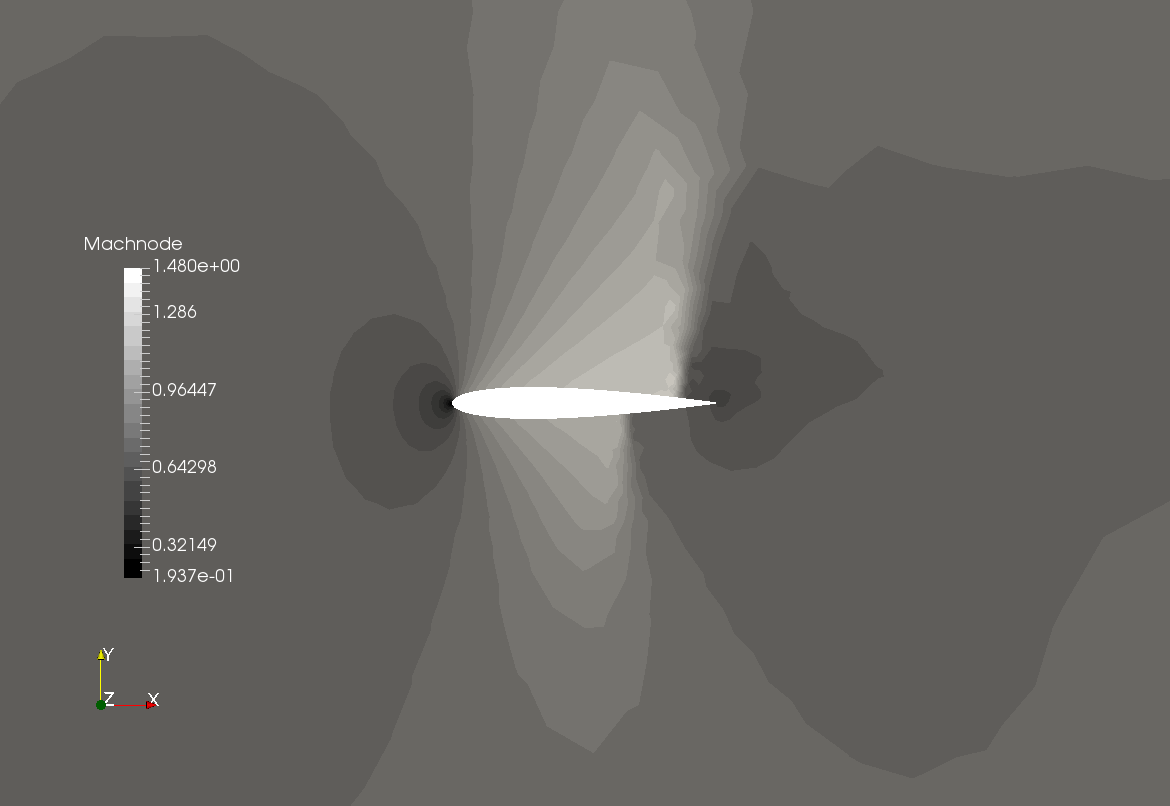
\includegraphics[width=0.4\linewidth]{41Mach_p0p1_naca}}
		\subfigure[Mach P0P1 with limiter]{%
			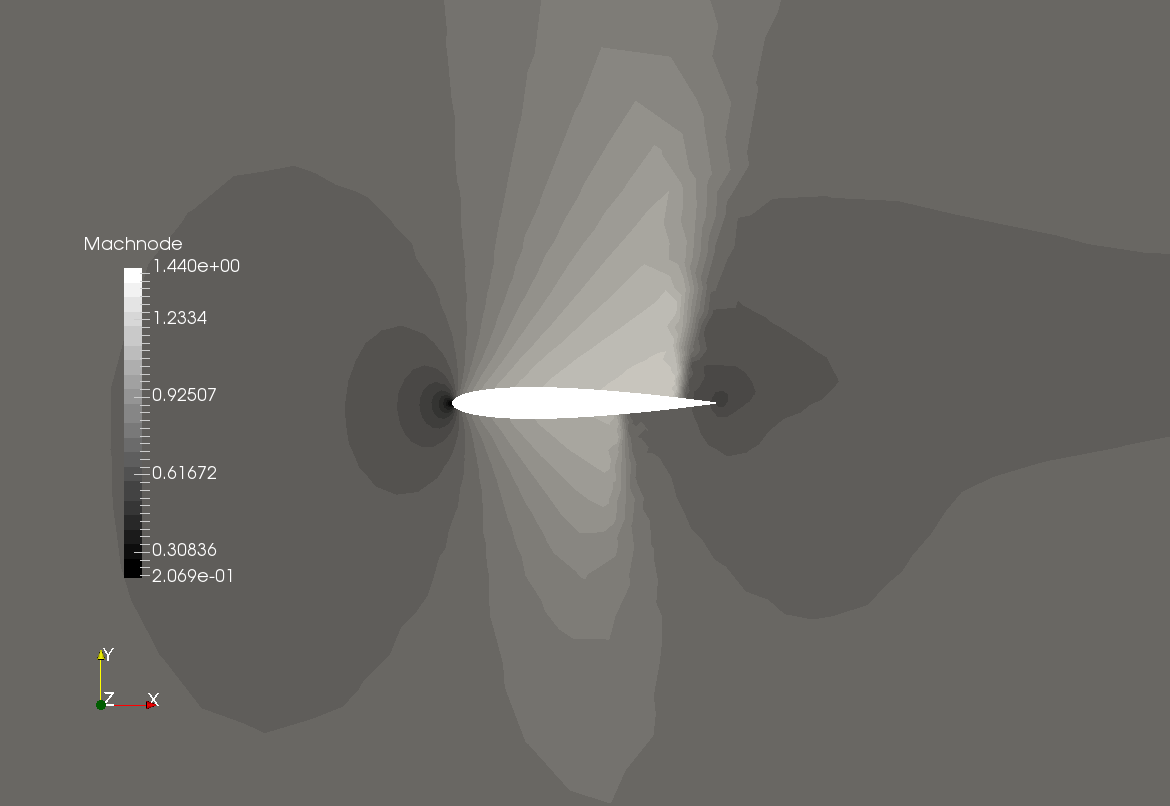
\includegraphics[width=0.4\linewidth]{42Mach_p0p1limi_naca}}
		\subfigure[Mach P0P1]{%
			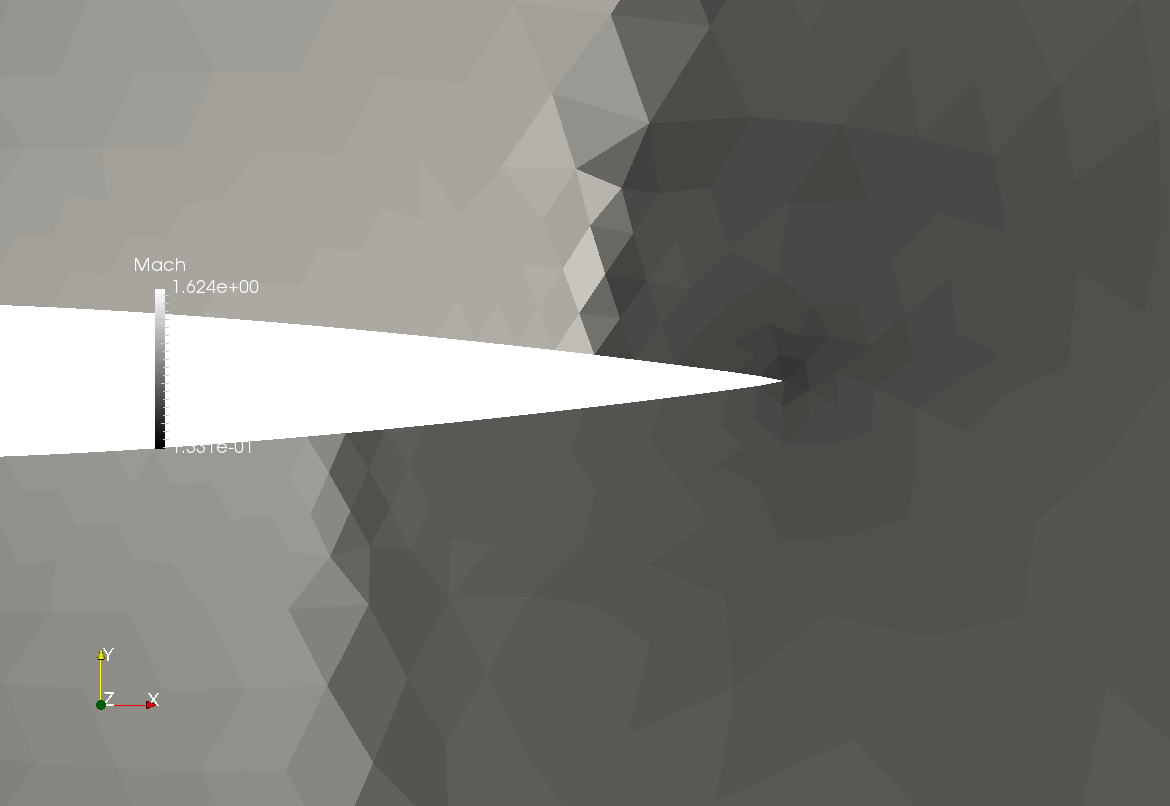
\includegraphics[width=0.4\linewidth]{zoomed_naca_nolimi}}
		\subfigure[Density P0P1 with Limiter]{%
			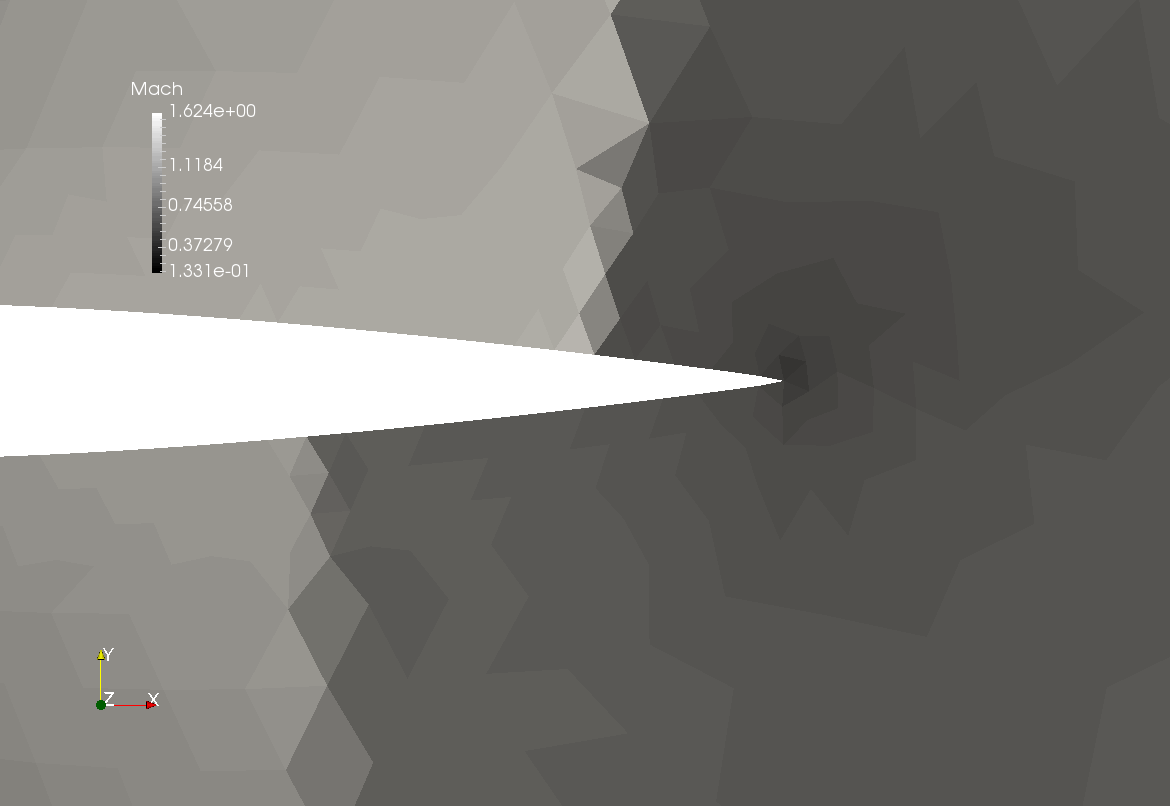
\includegraphics[width=0.4\linewidth]{zoomed_naca_limi}}
		%
		\caption{Solution of NACA airfoil}
		\label{figure9}
	\end{figure}
	\clearpage
	
	Fig. \ref{figure10} shows the convergence plot for all the three methods for airfoil. It is observed that the P0 takes least number of iterations and P1 with limiter takes most number of iterations.
	
	\begin{figure}[ht]
		\centering
		\subfigure[Absolute Residue]{%
			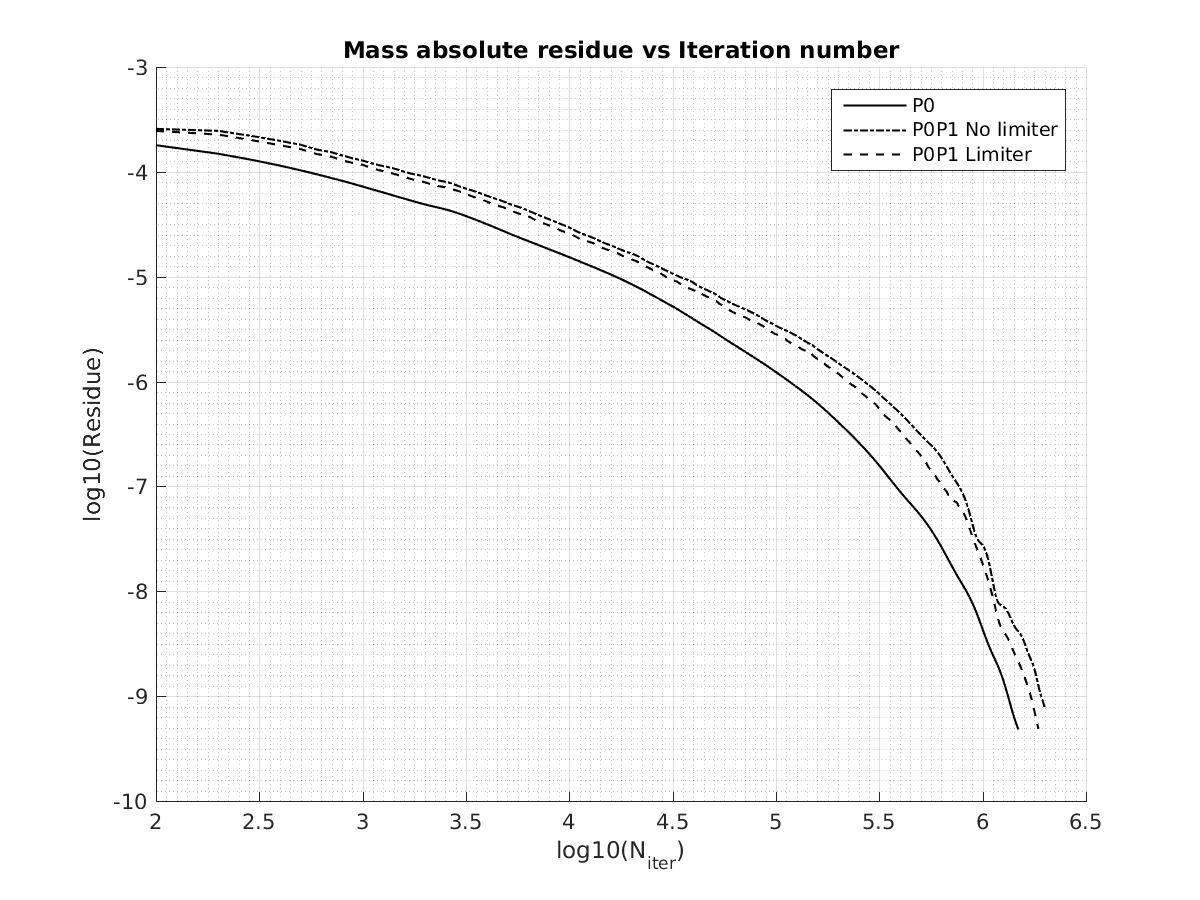
\includegraphics[width=0.45\linewidth]{43naca_abs_res}}
		\subfigure[Relative Residue]{%
			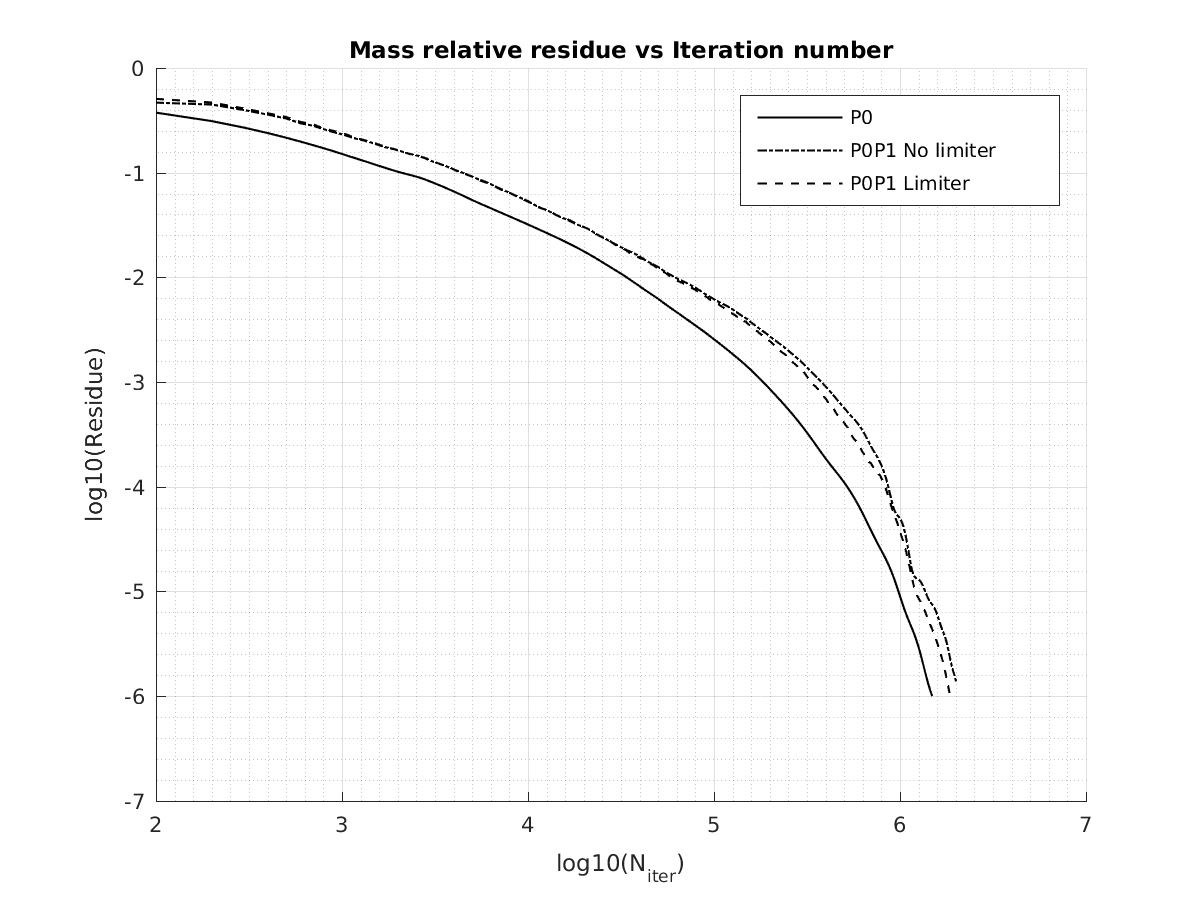
\includegraphics[width=0.45\linewidth]{44naca_rel_res}}
		\caption{Comparision of Residues for Naca airfoil}
		\label{figure10}
	\end{figure}
	\clearpage
	
	\subsection{Supersonic flow in a channel(M=1.1)}
	In the third case, internal flow over a circular bump with inlet Mach number of 1.1 is simulated with p0, reconstructed P0P1 without limiter and with limiter. Fig. \ref{bumpfig} shows the mesh of the channel. 
	
	\begin{figure}[ht]
		\centering
		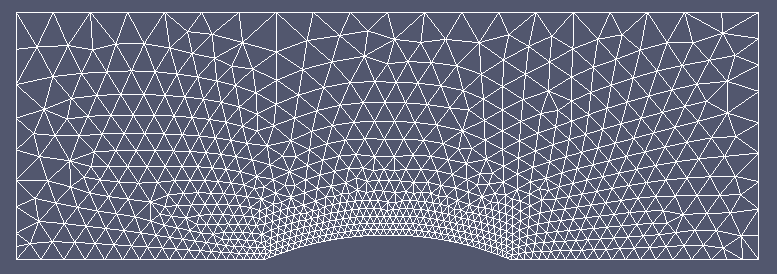
\includegraphics[width=1\linewidth]{bum_mesh_png}
		\caption{Comparision of flow inside internal flow}
		\label{bumpfig}
	\end{figure}
	
	It is observed that the case without limiter does not converge because of the huge oscillation in solution for supersonic Mach number and hence the results without limiter is not reported. Fig. \ref{figure8} shows the comparison of pressure, density and Mach number contours for internal flow with P0 and reconstructed P0P1 method with limiter. It can observed that the Mach number at the inlet is subsonic despite the supersonic inflow. This is because the shock wave occurs just before the entrance as there is decrease in cross-section at the bump.\newline
	\newline
	The Mach number continuously increase from the entrance to the bump, as the cross section is decreasing and the Mach number decreases downstream the bump followed by a shock at the corner because of the geometric singularity. Form the figure, it can be observed that the accuracy increases with reconstruction and sharp gradients can be seen across the shock. However, there are oscillation at the upper surface near the shock due to reconstruction despite using limiter.
	\clearpage
	
	\begin{figure}[ht]
		\centering
		\subfigure[P0]{%
			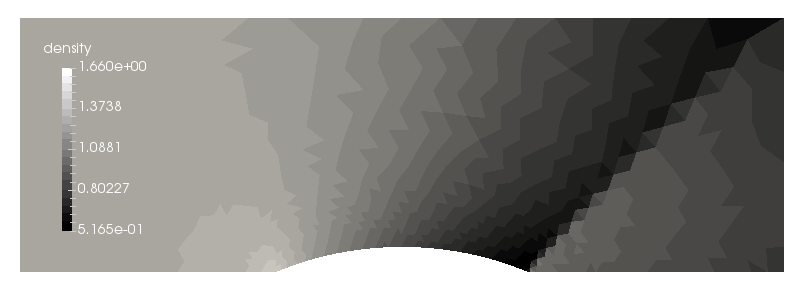
\includegraphics[width=0.7\linewidth]{28Density_bump_p0}}
		\subfigure[P0P1 Limiter]{%
			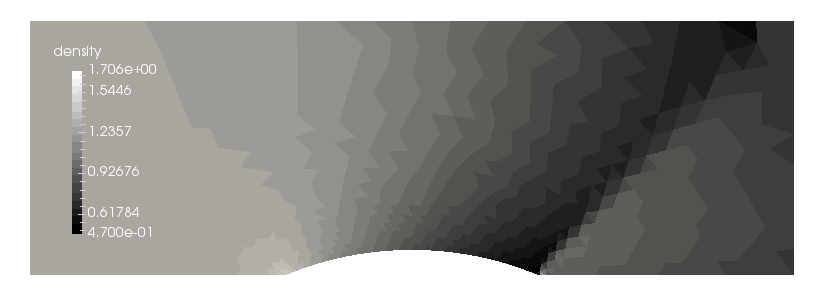
\includegraphics[width=0.7\linewidth]{29density_bump_p0_limi}}
		\subfigure[P0]{%
			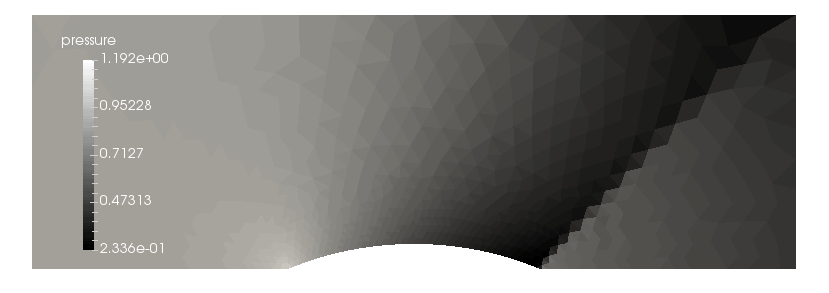
\includegraphics[width=0.7\linewidth]{30pres_bump_p0}}
		\subfigure[P0P1 limiter]{%
			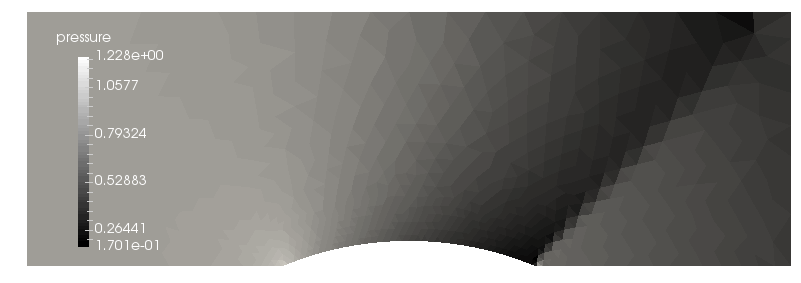
\includegraphics[width=0.7\linewidth]{31pres_bump_p0_limi}}
		\subfigure[P0]{%
			\includegraphics[width=0.7\linewidth]{32Mach_bump_p0}}
		\subfigure[P0P1 Limiter]{%
			\includegraphics[width=0.7\linewidth]{33Mach_bump_p0_limi}}
		%
		\caption{Comparision of flow inside internal flow}
		\label{figure8}
	\end{figure}
	
	\clearpage
	\section{Conclusion}
	In conclusion, the C++ program to solve Euler equation is successfully tested on three different cases with four discretization methods. From the subsonic flow past a cylinder simulation, the order of accuracy for reconstructed P0(Finite Volume) method is determined to be first order, P0P1 method without the limiter is second order accurate. It was observed that the reconstruction induces oscillation for higher Mach numbers and to avoid it Van-Alberta limiter has been introduced. However the order of accuracy of reconstruction with limiter decreases. To improve the accuracy, P1 method has been implemented but the order of accuracy has not been achieved because of a bug in the program.In the second test case, program is successfully tested on transonic flow past an airfoil and results looks to be promising. Finally supersonic flow inside a channel has been modelled and the reconstructed case without limiter did not converge because of the oscillations in the solution. It is observed that the oscillations in the solutions can be reduced by using a limiter and it is found that the simulation converged successfully with limiter.
	
	\section{Future Work}
	In this project, P1 method has been implemented to test the capability of DG method but the accuracy found to be reduced due to a bug in the program. Implementing the DGP1 method would be promising and it would give the second order solution without the effect of numerical oscillations when using reconstruction for higher Mach number.
	
	
	
	
	
	%% The Appendices part is started with the command \appendix;
	%% appendix sections are then done as normal sections
	%% \appendix
	
	%% \section{}
	%% \label{}
	
	%% References
	%%
	%% Following citation commands can be used in the body text:
	%% Usage of \cite is as follows:
	%%   \cite{key}          ==>>  [#]
	%%   \cite[chap. 2]{key} ==>>  [#, chap. 2]
	%%   \citet{key}         ==>>  Author [#]
	
	%% References with bibTeX database:
	
	\bibliographystyle{model1-num-names}
	\bibliography{sample.bib}
	
	%% Authors are advised to submit their bibtex database files. They are
	%% requested to list a bibtex style file in the manuscript if they do
	%% not want to use model1-num-names.bst.
	
	%% References without bibTeX database:
	
	% \begin{thebibliography}{00}
	
	%% \bibitem must have the following form:
	%%   \bibitem{key}...
	%%
	
	% \bibitem{}
	
	% \end{thebibliography}
	
	
\end{document}

%%
%% End of file `elsarticle-template-1-num.tex'.
